% cap4.tex

\chapter{Análisis de Resultados}
\label{c4} % la etiqueta para referencias


\section{Resultados Replicación modelo original}\label{replicaciongams}

\begin{table}[H]
    \centering
    \begin{tabular}{|l|l|l|l|l|l|l|}
    \hline
        CAP &  $\theta$ & $\pi^a$ & Ingreso &  Año Carbón & $ \pi^v$   \\ \hline
        100,000,000  & 100,000,000  &  \$315.82  &  \$31,582,452,378.43  & 2020 &  \$315.82   \\ \hline
        200,000,000  & 200,000,000  &  \$183.55  &  \$36,710,421,141.24  & 2025 &  \$183.55   \\ \hline
        300,000,000  & 300,000,000  &  \$138.02  &  \$41,404,754,716.75  & 2028 &  \$138.02   \\ \hline
        400,000,000  & 400,000,000  &  \$110.19  &  \$44,074,042,301.57  & 2031 &  \$110.19   \\ \hline
        500,000,000  & 500,000,000  &  \$92.93  &  \$46,465,119,507.96  & 2035 &  \$92.93   \\ \hline
        600,000,000  & 600,000,000  &  \$79.43  &  \$47,656,975,707.52  & 2038 &  \$79.43   \\ \hline
        700,000,000  & 700,000,000  &  \$68.65  &  \$48,056,890,569.06  & 2040 &  \$68.65   \\ \hline
        800,000,000  & 800,000,000  &  \$59.49  &  \$47,589,690,505.72  & 2042 &  \$59.49   \\ \hline
        900,000,000  & 900,000,000  &  \$52.44  &  \$47,194,995,047.68  & 2050 &  \$52.44   \\ \hline
        1,000,000,000  & 1,000,000,000  &  \$46.66  &  \$46,660,328,771.21  & 2050 &  \$46.66   \\ \hline
    \end{tabular}
    \caption{{\footnotesize Resultados Modelo Original}}
    \label{resultadosmodelooriginal}
\end{table}

\section{Determinación parámetros de los modelos nuevos}\label{introresultados}

En el capítulo anterior se aplica el concepto de atención racional en el modelo del subastador. Basada en \cite{dewan_estimating_2020}, se agrega un rendimiento de obtención de ingreso (en este caso el ingreso del subastador es la venta de permisos en la primera etapa), dependiente de cuanto dinero gasta en información adicional. Finalmente, se aplica el concepto de atención (inatención) racional en dos versiones: \textit{Profit Oriented} \ref{profit} y Bienestar Social \ref{bienestarsocial}. 
\vspace{2.5mm}

Para completar los modelos, se deben agregar los parámetros de estos, los cuales están definidos en la Figura \ref{fig:nomenclatura1}, sobre costos, capacidades instaladas, demanda energética en cada periodo, factores de contaminación por tecnología, entre otros. Para esta nueva estructuración del modelo de \textit{cap and trade}, se repetirán los valores de los parámetros aplicados en el modelo original de \cite{amigo_two_2021}. Sus valores específicos se encuentran en el Anexo \ref{anexo:parametros}.
\vspace{2.5mm}

Para utilización de los nuevos parámetros $d$ y $c$ (información pública y costo marginal de información ) se hacen los siguientes supuestos para cada uno de ellos.
\vspace{2.5mm}

Por un lado,  el parámetro $d$ de información disponible se determina considerando que esta información es equivalente al error de cálculo de los presupuestos de carbono realizados para el NDC chileno. Este supuesto se hizo ya que tiene sentido en cuanto al trabajo que debe realizar el subastador para aumentar sus ganancias y encontrar un beneficio social mayor. Invertir por disminuir el ruido (o error) de determinación de presupuesto de carbono, para generar un mayor beneficio social y económico, es necesario invertir en la obtención de información que disminuya este ruido. \vspace{2.5mm}

Para determinar este error, debido a que no se encontró información sobre cómo se calculó el presupuesto de $1.100\quad MTCO_{2}e$ establecido en el NDC actualizado de Chile para el periodo 2020-2030 por el Ministerio del Medio Ambiente de Chile, se utilizó un estudio sobre el cálculo de estos presupuestos.
\vspace{2.5mm}

Los autores \citeB{andres_new_2014} estudian este cálculo y la existencia de un error en ellos. Proponen, debido a diferentes circunstancias y características de cada país, un error estimado del cálculo de estos parámetros. Señalando que existe un error en Chile de 0,202. Con esto, se toma un valor de información pública o información disponible $d=0,798$, el cuál representa el total del valor del presupuesto de carbono determinado por Chile que sí es confiable o sí representa una estimación real del presupuesto que se debe considerar.   
\vspace{2.5mm}

A partir de este presupuesto, es trabajo del subastador minimizar el ruido y encontrar un presupuesto que maximice sus ganancias y, consecuentemente, maximice el bienestar social.
\vspace{2.5mm}

Para un estudio complementario a cómo este error puede afectar las emisiones de un país y la importancia de ofrecer un intervalo de confianza, o mencionar el error de los cálculos en algo como el presupuesto de carbono, se recomienda la lectura del trabajo de  \citeB{ballantyne_audit_2015}.
\vspace{2.5mm}

Por otro lado, el valor del parámetro $c$, se determina por medio de una calibración de cada modelo, variando este parámetro hasta calibrar cada uno con el modelo original. En otras palabras, se toma como referencia la solución del modelo original para un presupuesto de carbono (parámetro exógeno al modelo)  dado de 100 millones de toneladas de $CO_{2}e$. Se toma el óptimo encontrado de la variable $\pi_a$ para calibrar el modelo. Entonces, se varía el parámetro $c$ en los modelos nuevos hasta obtener un precio de venta de permisos por parte del subastador (representado por la variable $\pi_a$ en los modelos) similar o igual al del modelo original para el mismo presupuesto de carbono.
\vspace{2.5mm}

El modelo original, con un presupuesto de 100$MtCO_{2}e$, encuentra un óptimo con la variable $\pi^a= \$315.83$.
\vspace{2.5mm}

A continuación, se calibran, resuelven, evalúan y analizan ambas versiones reestructuradas del modelo original.

\section{Modelo \textit{Profit Oriented}} \label{resultadosprofit}

El modelo propuesto en el capítulo \ref{profit} se traduce en el siguiente problema de equilibrio en formato MCP: 

\textbf{MCP productor}

\begin{footnotesize}
\begin{align}
    0 \leq x_i(0) \perp (I_i  + \sum_{\omega}\psi_{i,\omega} -\sum_{\omega, t>0} \alpha_{i,\omega,t}(CF_i\cdot \tau)) \geq 0 \qquad \forall \  i \\
    0 \leq x_i(t,\omega) \perp (Pr(\omega) \Bigg[\frac{1}{(1+R)^t}TCR_i(t) \cdot I_i \Bigg] - \sum_{t> t\prime}\alpha_{i,\omega,t} ( CF_i \cdot \tau)+ \psi_{i,\omega}) \geq 0\\
    0 \leq Q_i(0) \perp ( \big(a_{i}+b_i Q_{i}(0)\big)-\pi^d(0) + \kappa_i  + \sum_{\omega} \gamma_{i,\omega}\varepsilon_i) \geq 0\\
    0 \leq Q_i(t,\omega) \perp (Pr(\omega)  \frac{1}{(1+R)^t} \bigg( TC_i(t) \big(a_{i}+b_i Q_i(t,\omega)\big ) -\pi^d(t,\omega) \bigg) + \alpha_{i,\omega,\tau} + \gamma_{i,\omega} \varepsilon_{i}) \geq 0 \qquad \forall \ i, \omega, t > 0\\
    0 \leq A_i \perp (\pi^{a} - \sum_{\omega}\beta_{i,\omega} - \sum_{\omega}\gamma_{i,\omega}) \geq 0 \qquad \forall  i\\
    0 \leq \cdot  V_i(w) \perp (-Pr(\omega) \pi^v(\omega) + \beta_{i,\omega}  + \gamma_{i,\omega})\geq 0 \qquad \forall \  i, \omega\\ 
   0 \leq  P_i(w) \perp (Pr(\omega) \pi^v(\omega) -\gamma_{i,\omega}) \geq  0  \qquad \forall \  i, \omega \\
     0 \leq \big(CF_i \cdot \tau \big) \Bigg[\bar{Q}_i + \sum_{t\leq t^{\prime}} x_i(t,\omega) + x_i(0) \Bigg] - Q_i(t,\omega)  \perp \alpha_{i,\omega,\tau} \geq 0 \qquad \forall \ i, \omega, t  > 0\\
     0 \leq \Big(CF_i\cdot\tau \Big)\bar{Q}_i(0)-Q_{i}(0) \perp \kappa_i \geq 0 \qquad \forall \ i \\
     0 \leq  A_{i} - V_i(\omega) \perp \beta_{i,\omega} \geq 0 \qquad \forall  \ \omega \\
     0 \leq  A_{i} + P_{i} (\omega) - V_i(\omega) - \sum_{t>0} Q_i(t,\omega) \varepsilon_{i} -Q_i(0)\varepsilon_{i} \perp \gamma_{i,\omega} \geq 0 \qquad \forall \ i, \omega\\
     0 \leq  RP_i - \bar{Q}_i - x_i(0) - \sum_{t>0} x_i(t,\omega) \perp \psi_{i,\omega} \geq 0 \qquad \forall \ i,\omega 
\end{align}
\end{footnotesize}

\textbf{MCP condiciones de mercado}

\begin{footnotesize}
\begin{align}
0 \leq \pi^a \perp \theta - \sum_{i}A_i= 0\\
0 \leq \pi^v(\omega) \perp \sum_{i}P_{i,\omega} - \sum_{i}V_{i,\omega} = 0 \qquad \forall \omega\\
0 \leq \pi^d(0) \perp \sum_{i}Q_i(0) - D(0)= 0\\
 0 \leq \pi^d(\omega,t) \perp \sum_{i}Q_i(t,\omega) - D(t,\omega) = 0 \qquad \forall \omega,t
\end{align}
\end{footnotesize}

\textbf{MCP subastador}

\begin{footnotesize}
\begin{align}
0\leq -P\pi^a(1+\eta) \perp \theta \geq 0 \label{compllag33}\\
0 \leq \theta \pi^a P - c(P-d)^2 \perp \eta \geq 0 \label{compllag331}
\end{align}
\end{footnotesize}

\subsection{Calibración del modelo}

Para realizar la calibración del modelo, se resuelve repetidas veces en el \textit{solver} variando únicamente el costo $c$ hasta encontrar un valor óptimo de $\pi^a $ similar al del modelo original para el CAP de 100 millones de $CO_{2}e$.     
\vspace{2.5mm}

En el Cuadro \ref{calibracionPO}, se observa que no se encuentran valores mayores a \$100. Esto es debido a las altas cantidades de permisos emitidos por el subastador. A mayor cantidad de permisos, menor será el precio debido a la ley de oferta y demanda.
\vspace{2.5mm}

\begin{table}[H]
    \centering
    \begin{tabular}{|l|l|l|l|l|l|}
    \hline
        c & $\pi^a$ & $\theta$ & $\pi^a$ original &  CAP& $\Delta \pi^a$  \\ \hline
         \$10  &  \$38.03  & 3.29E+08 &  \$315.83  & 1.00E+08 &  \$-277.80   \\ \hline
         \$50  &  \$43.13  & 2.97E+08 &  \$315.83  & 1.00E+08 &  \$-272.69   \\ \hline
         \$500  &  \$38.47  & 3.31E+08 &  \$315.83  & 1.00E+08 &  \$-277.35   \\ \hline
         \$5,000  &  \$38.25  & 3.33E+08 &  \$315.83  & 1.00E+08 &  \$-277.57   \\ \hline
         \$50,000  &  \$30.57  & 7.95E+08 &  \$315.83  & 1.00E+08 &  \$-285.26   \\ \hline
         \$500,000  &  \$28.29  & 8.46E+08 &  \$315.83  & 1.00E+08 &  \$-287.54   \\ \hline
         \$5,000,000  &  \$27.96  & 8.53E+08 &  \$315.83  & 1.00E+08 &  \$-287.87   \\ \hline
         \$50,000,000  &  \$28.64  & 8.39E+08 &  \$315.83  & 1.00E+08 &  \$-287.18   \\ \hline
         \$500,000,000  &  \$27.66  & 8.59E+08 &  \$315.83  & 1.00E+08 &  \$-288.17   \\ \hline
         \$5,000,000,000  &  \$27.91  & 8.54E+08 &  \$315.83  & 1.00E+08 &  \$-287.92   \\ \hline
         \$10,000,000,000  &  \$27.00  & 8.60E+08 &  \$315.83  & 1.00E+08 &  \$-288.83   \\ \hline
         \$50,000,000,000  &  \$28.18  & 8.49E+08 &  \$315.83  & 1.00E+08 &  \$-287.65   \\ \hline
         \$100,000,000,000  &  \$27.71  & 8.58E+08 &  \$315.83  & 1.00E+08 &  \$-288.11   \\ \hline
         \$200,000,000,000  &  \$25.16  & 9.22E+08 &  \$315.83  & 1.00E+08 &  \$-290.67   \\ \hline
         \$300,000,000,000  &  \$28.00  & 8.53E+08 &  \$315.83  & 1.00E+08 &  \$-287.82   \\ \hline
         \$450,000,000,000  &  \$26.51  & 8.87E+08 &  \$315.83  & 1.00E+08 &  \$-289.32   \\ \hline
         \$500,000,000,000  &  \$33.36  & 6.12E+08 &  \$315.83  & 1.00E+08 &  \$-282.47   \\ \hline
         \$5,000,000,000,000  &  \$-  & 1.29E+09 &  \$315.83  & 1.00E+08 &  \$-315.83   \\ \hline
         \$50,000,000,000,000  &  \$-  & 5.87E+09 &  \$315.83  & 1.00E+08 &  \$-315.83   \\ \hline
    \end{tabular}
    \caption{{\footnotesize Calibración modelo Profit Oriented}}
    \label{calibracionPO}
\end{table}

Para entender por qué se emiten tantos permisos para cada costo, basta con observar que falta restringir la cantidad de permisos que se pueden emitir. El subastador busca únicamente maximizar sus utilidades, por lo que siempre emitirá la mayor cantidad de permisos posibles para así vender más y producir más ganancias. La única restricción que tienen estos permisos es la de no producir más permisos que los necesarios para abastecer la demanda de electricidad en el futuro. Entonces, con este formato, se emitirá la cantidad de permisos necesarios para abastecer esta demanda con la contaminación que esta produce.
\vspace{2.5mm}

En consecuencia a lo analizado y debido a que producir con fuentes no renovables es más rentable, el modelo hace que se emita la cantidad de permisos que las empresas de generación contaminantes necesitarán para abastecer la demanda. 
\vspace{2.5mm}

Con el fin de resolver el problema anterior, ya que el objetivo de este trabajo es encontrar un modelo que minimice las emisiones de carbono y aumente la inversión en energías renovables, se debe restringir la cantidad de permisos a emitir respecto al CAP.


\subsection{Resultados}

NO CREO QUE DEBA INCUIR ESTO 

A pesar de lo anterior, se utiliza este modelo para tener una idea inicial de cómo responde el subastador al cambio exógeno del rendimiento.

Con esto, al correr el modelo en el \textit{solver}, cambiando únicamente el valor del rendimiento ($P$), se encontraron los siguientes resultados:

\begin{table}[H]
\centering
\begin{tabular}{|l|l|l|}
\hline
\textbf{P($\%$)} & \textbf{$\theta$ (millones)} & \textbf{$\pi^a$($\frac{\$}{\theta}$)} \\ \hline
20 & 3203 & 0 \\ \hline
25 & 190 & 103.196 \\ \hline
30 & 204.63 & 73.335 \\ \hline
35 & 219.81 & 77.973 \\ \hline
40 & 219.79 & 60.880 \\ \hline
45 & 235.31 & 60.448 \\ \hline
50 & 379.72 & 77.507 \\ \hline
55 & 221.79 & 52.927 \\ \hline
60 & 230.75 & 48.799 \\ \hline
65 & 239.28 & 46.123 \\ \hline
70 & 248.33 & 49.598 \\ \hline
75 & 225.99 & 47.855 \\ \hline
80 & 235.93 & 62.802 \\ \hline
85 & 263.95 & 42.426 \\ \hline
90 & 272.16 & 41.955 \\ \hline
95 & 275.08 & 39.492 \\ \hline
100 & 328.44 & 38.110 \\ \hline
\end{tabular}
\caption{{\footnotesize Resultados modelo con restricción de rendimiento}}
\label{tabla:conrestrrend}
\end{table}

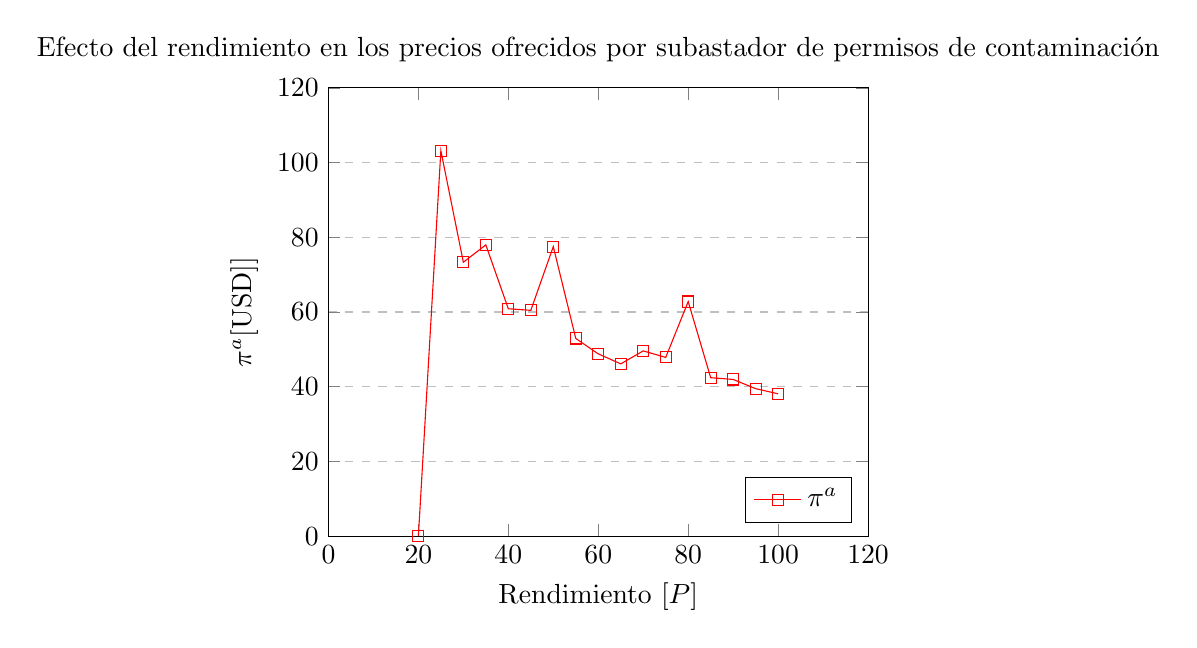
\begin{tikzpicture}
\begin{axis}[
    title={Efecto del rendimiento en los precios ofrecidos por subastador de permisos de contaminación},
    xlabel={Rendimiento [$P$]},
    ylabel={$\pi^a$[USD]]},
    xmin=0, xmax=120,
    ymin=0, ymax=120,
    xtick={0,20,40,60,80,100,120},
    ytick={0,20,40,60,80,100,120},
    legend pos=south east,
    ymajorgrids=true,
    grid style=dashed,
]

\addplot[
    color=red,
    mark=square,
    ]
    coordinates {
    (20,0)(25,103.196)(30,73.335)(35,77.973)(40,60.880)(45,60.448)(50,77.507)(55,52.927)(60,48.799)(65,46.123)(70,49.598)(75,47.855)(80,62.802)(85,42.426)(90,41.955)(95,39.492)(100,38.110)
    };
    \legend{$\pi^a$}
    
\end{axis}
\end{tikzpicture}

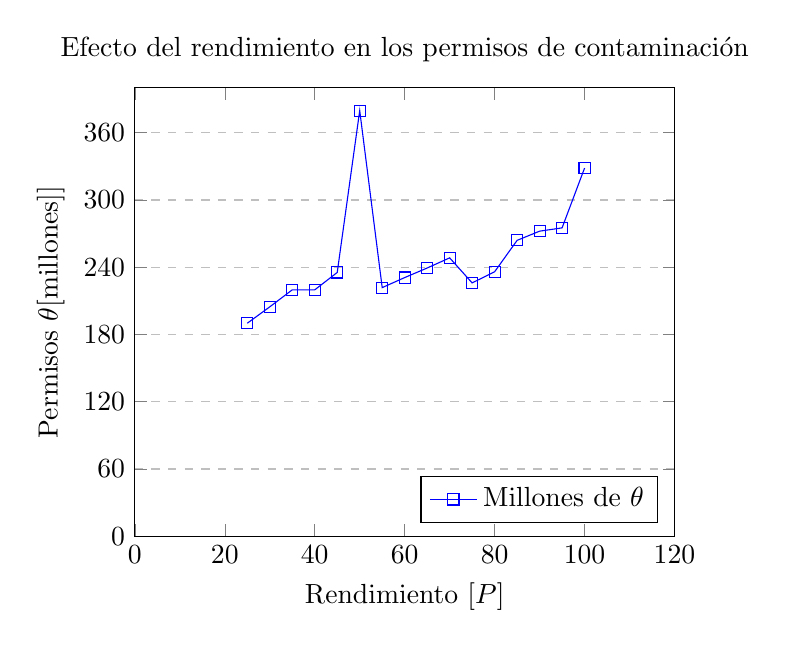
\begin{tikzpicture}
\begin{axis}[
    title={Efecto del rendimiento en los permisos de contaminación},
    xlabel={Rendimiento [$P$]},
    ylabel={Permisos $\theta$[millones]]},
    xmin=0, xmax=120,
    ymin=0, ymax=400,
    xtick={0,20,40,60,80,100,120},
    ytick={0,60,120,180,240,300,360},
    legend pos=south east,
    ymajorgrids=true,
    grid style=dashed,
]

\addplot[
    color=blue,
    mark=square,
    ]
    coordinates {
    (25,190)(30,204.63)(35,219.81)(40, 219.79)(45, 235.31)(50,379.72)(55,221.79)(60, 230.75)(65,239.28)(70,248.33)(75,225.99)(80,235.93 )(85,263.95)(90,272.16)(95,275.08)(100,328.44)
    };
    \legend{Millones de $\theta$}
    
\end{axis}
\end{tikzpicture}

\subsection{Adaptación modelo \textit{Profit Oriented}}

\begin{footnotesize}
\begin{equation}
\begin{array}{rrclcl}
   \displaystyle \min_{\theta} & -\theta \pi^aP + c(P-d)^2+F(\theta) \\\textrm{s.a.} \label{eq:profit2}\\
\end{array}
\end{equation}
\begin{equation}
\begin{array}{cl}
    \theta \pi^a P - c(P-d)^2 \geq 0 & (\eta)  \label{profit2:r1}
\end{array}
\end{equation}
\begin{equation}
\begin{array}{cl}
    \hat{\theta}\cdot(1+error)-\theta \geq 0 & (\mu)  \label{profit2:r2}
\end{array}
\end{equation}
\begin{equation}
\begin{array}{cl}
    \theta \geq 0 & (\varrho)
\end{array}
\end{equation}
\end{footnotesize}

La incorporación de la restricción \ref{profit2:r2}, tiene como fin restringir la emisión de permisos incorporando el CAP. Los permisos se acotan a que estos no pueden superar el CAP mas su error de cálculo explicado anteriormente.
\vspace{2.5mm}

$\hat{\theta}$ toma el valor del presupuesto de emisiones (CAP) impuesto por el gobierno. En esta misma restricción, se utiliza el valor error, el cuál representa el error de cálculo de este presupuesto, estimado por \cite{andres_new_2014}. Definiendo un $error=0,202$. 
\vspace{2.5mm}

Con esta nueva formulación, se calibra el modelo y posteriormente se resuelve.

\subsection{Calibración}

Para calibrar, se realiza el mismo procedimiento explicado anteriormente. 

\begin{table}[H]
    \centering
    \begin{tabular}{|l|l|l|l|l|l|}
    \hline
        c & $\pi^a$ & $\theta$ & $\pi^a$ original &  CAP& $\Delta \pi^a$  \\ \hline
         \$5  &  \$270.13  & 1.20E+08 &  \$315.83  & 1.00E+08 &  \$45.70   \\ \hline
         \$5,000  &  \$241.47  & 1.20E+08 &  \$315.83  & 1.00E+08 &  \$74.36   \\ \hline
         \$50,000  &  \$239.26  & 1.20E+08 &  \$315.83  & 1.00E+08 &  \$76.57   \\ \hline
         \$500,000  &  \$223.70  & 1.20E+08 &  \$315.83  & 1.00E+08 &  \$92.12   \\ \hline
         \$5,000,000  &  \$226.19  & 1.20E+08 &  \$315.83  & 1.00E+08 &  \$89.64   \\ \hline
         \$50,000,000  &  \$270.13  & 1.20E+08 &  \$315.83  & 1.00E+08 &  \$45.70   \\ \hline
         \$500,000,000  &  \$270.13  & 1.20E+08 &  \$315.83  & 1.00E+08 &  \$45.70   \\ \hline
         \$5,000,000,000  &  \$260.94  & 1.20E+08 &  \$315.83  & 1.00E+08 &  \$54.89   \\ \hline
         \$50,000,000,000  &  \$17.56  & 1.16E+08 &  \$315.83  & 1.00E+08 &  \$298.26   \\ \hline
         \$500,000,000,000  &  \$172.70  & 1.18E+08 &  \$315.83  & 1.00E+08 &  \$143.13   \\ \hline
         \$900,000,000,000  &  \$310.34  & 1.18E+08 &  \$315.83  & 1.00E+08 &  \$5.49   \\ \hline
         \$910,000,000,000  &  \$313.76  & 1.18E+08 &  \$315.83  & 1.00E+08 &  \$2.07   \\ \hline
         \$912,000,000,000  &  \$314.12  & 1.18E+08 &  \$315.83  & 1.00E+08 &  \$1.70   \\ \hline
         \$915,000,000,000  &  \$328.58  & 1.14E+08 &  \$315.83  & 1.00E+08 &  \$12.75   \\ \hline
         \$920,000,000,000  &  \$317.24  & 1.18E+08 &  \$315.83  & 1.00E+08 &  \$1.41   \\ \hline
         \$1,000,000,000,000  &  \$346.94  & 1.18E+08 &  \$315.83  & 1.00E+08 &  \$31.11   \\ \hline
         \$2,000,000,000,000  &  \$724.72  & 1.13E+08 &  \$315.83  & 1.00E+08 &  \$408.90   \\ \hline
         \$3,000,000,000,000  &  \$1,087.10  & 1.13E+08 &  \$315.83  & 1.00E+08 &  \$771.27   \\ \hline
         \$4,000,000,000,000  &  \$2,218.81  & 7.38E+07 &  \$315.83  & 1.00E+08 &  \$1,902.98   \\ \hline
    \end{tabular}
    \caption{{\footnotesize Calibración modelo Profit Oriented 2}}
    \label{calibracionPO2}
\end{table}

En el Cuadro \ref{calibracionPO2} se observa que existe un efecto lineal entre el costo $c$ y los precios $\pi^a$ a partir de los $\$50.000.000.000$ en costos. Esto se explica gracias a como este modelo está formulado: a mayor costo, se incurrirá a un mayor precio en los permisos para tener utilidades positivas. Antes del precio mencionado, los costos no son lo suficientemente altos como para afectar las ganancias.
\vspace{2.5mm}

Finalmente, con un costo $c= \$ 920,000,000,000$ se tiene la mejor aproximación al $\pi^a$ original. 
\vspace{2.5mm}

\subsection{Resultados}

En este modelo se incorpora el rendimiento como parámetro, por lo que se estudia como afecta las variables del modelo.
\vspace{2.5mm}

\begin{table}[H]
    \centering
    \begin{tabular}{|l|l|l|l|l|}
    \hline
        Rend[P]  & CAP & $\theta$  & $\frac{\theta}{CAP}$  & $\pi^a$  \\ \hline
        0.798  & 100,000,000  & 120,200,000 & 1.20  &  \$270.13   \\ \hline
        0.8  & 100,000,000 & 120,200,000 & 1.20  &  \$270.13   \\ \hline
        0.85  & 100,000,000 & 113,654,321 & 1.14  &  \$25.75   \\ \hline
        0.9  & 100,000,000 & 113,568,965 & 1.14  &  \$93.65   \\ \hline
        0.95  & 100,000,000 & 118,470,479 & 1.18  &  \$188.86   \\ \hline
        0.99  & 100,000,000 & 114,916,396 & 1.15  &  \$298.11   \\ \hline
        1  & 100,000,000 & 118,332,486 & 1.18  &  \$317.24   \\ \hline
    \end{tabular}
    \caption{{\footnotesize Efecto de $P$ en $\theta$ y $\pi^a$}}
    \label{efectopenthetapia}
\end{table}


En el Cuadro \ref{efectopenthetapia} se mantiene el presupuesto constante para entender el efecto del rendimiento en los permisos emitidos ($\theta$) y los precios establecidos por el subastador ($\pi^a$) al mantener constante el presupuesto de carbono (CAP). 
\vspace{2.5mm}

Por un lado, estos resultados muestran un efecto triangular en los permisos emitidos, con bajos rendimientos, se emite el máximo de permisos ($CAP + error$), en los rendimientos medios (0.85,0.9) se encuentra un mínimo de permisos emitidos y finalmente, con el rendimiento máximo, los permisos vuelven a subir cercano a $CAP + error$.
\vspace{2.5mm}

Por otro lado, existe un efecto similar en los precios $\pi^a$, encontrando valores máximos en los extremos del rendimiento.
\vspace{2.5mm}

De ambas observaciones se concluye que en los rendimientos 0.85 y 0.9 existe una inclinación a generar menores utilidades (menor ingresos debido al precio de permisos) y se busca un mejor bienestar social (se emiten menos permisos, o sea, se contamina menos).
\vspace{2.5mm}

Los resultados para todos los presupuesto de carbono se encuentran en el Cuadro \ref{efectopenthetapiatodoCAP} del Anexo \ref{anexoPO}.
\vspace{2.5mm}

\begin{table}[H]
    \centering
    \begin{tabular}{|l|l|l|l|l|}
    \hline
        Rend[P]  & CAP & $\theta$  & $\frac{\theta}{CAP}$  & $\pi^a$  \\ \hline
         0.8 & 100,000,000 & 120,200,000 & 1.20 &  \$270.13   \\ \hline
        0.8 & 200,000,000 & 240,400,000 & 1.20 &  \$60.57   \\ \hline
        0.8 & 300,000,000 & 360,600,000 & 1.20 &  \$119.47   \\ \hline
        0.8 & 400,000,000 & 454,798,037 & 1.14 &  \$95.83   \\ \hline
        0.8 & 500,000,000 & 601,000,000 & 1.20 &  \$79.31   \\ \hline
        0.8 & 600,000,000 & 605,279,899 & 1.01 &  \$66.57   \\ \hline
        0.8 & 700,000,000 & 605,279,899 & 0.86 &  \$56.37   \\ \hline
        0.8 & 800,000,000 & 961,600,000 & 1.20 &  \$152.50   \\ \hline
        0.8 & 900,000,000 & 605,279,899 & 0.67 &  \$42.26   \\ \hline
        0.8 & 1,000,000,000 & 605,279,899 & 0.61 &  \$35.98   \\ \hline
    \end{tabular}
    \caption{{\footnotesize Efecto del $CAP$ en $\theta$ y $\pi^a$}}
    \label{efectocapthetapia}
\end{table}
\vspace{2.5mm}

En el Cuadro \ref{efectocapthetapia} se muestra, manteniendo el rendimiento constante, el efecto del cambio del parámetro CAP en los permisos emitidos y los precios de permisos $\pi^a$.  Se observa que a mayor CAP existe un menor número de permisos emitidos relativos al CAP. En otras palabras, $\frac{\theta}{CAP}$ disminuye mientras mayor es el CAP establecido por el gobierno.
\vspace{2.5mm}

En adición a lo anterior, los precios $\pi^a$ tienen un comportamiento sinusoidal, tal vez ruido blanco, respecto al cambio en el CAP. Por un lado, se puede observar una tendencia a la baja para el precio mientras sube la cantidad de permisos (la ley de oferta y demanda espera esto ), pero, existen saltos extraños como en el CAP$=800MtCO_2$, donde se emiten muchos permisos y los precios aumentan. Estas anomalías pueden ser debido a que en estas ocasiones se invirtió más en información, traspasando los costos a la empresas que compran los permisos.
\vspace{2.5mm}

Los resultados para todos los rendimientos se encuentran en el Cuadro \ref{efectopenthetapiatodoCAP} del Anexo \ref{anexoPO}.
\vspace{2.5mm}

La Figura \ref{rendcap} muestra la relación entre la variación del CAP y el cociente de los permisos emitidos y el CAP para todos los rendimientos (recordar que en este modelo estos son parámetros).
\vspace{2.5mm}

\begin{figure}[H]
\centering
\resizebox{12cm}{10cm}{%
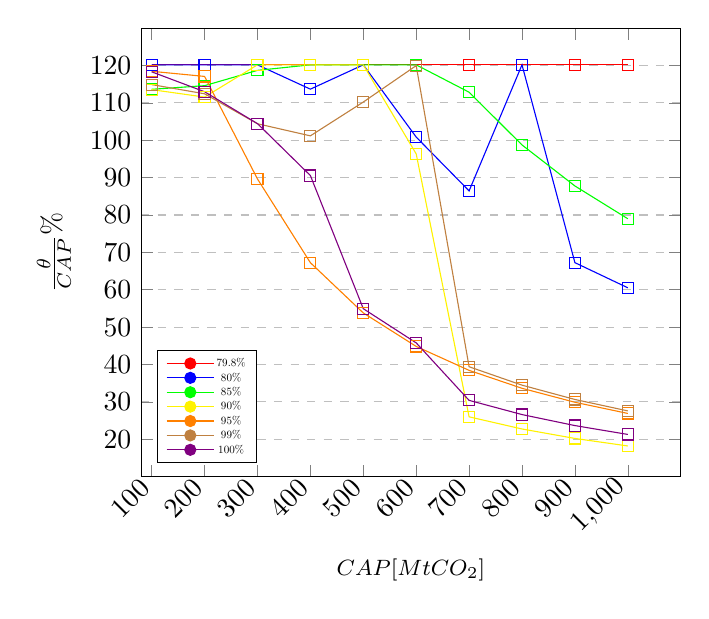
\begin{tikzpicture}
\centering
\begin{axis}[legend style={nodes={scale=0.4, transform shape}}, 
        legend image post style={mark=*},
    xlabel={{\footnotesize $CAP[MtCO_2]$}},
    ylabel={$\frac{\theta}{CAP}\%$},
    xmin=80, xmax=1100,
    ymin=10, ymax=130,
    xtick={100,200,300,400,500,600,700,800,900,1000},
    xticklabel style = {rotate=45,anchor=east},
    ytick={20,30,40,50,60,70,80,90,100,110,120},
    legend pos=south west,
    ymajorgrids=true,
    grid style=dashed,
]

\addplot[
    color=red,
    mark=square,
    ]
    coordinates {
    (100,120.2)(200,120.2)(300,120.2)(400,120.2)(500,120.2)(600,120.2)(700,120.2)(800,120.2)(900,120.2)(1000,120.2)
    };

\addplot[
    color=blue,
    mark=square,
    ]
    coordinates {
    (100,120.2)(200,120.2)(300,120.2)(400,113.69)(500,120.2)(600,100.87)(700,86.46)(800,120.2)(900,67.25)(1000,60.52)
    };
\addplot[
    color=green,
    mark=square,
    ]
    coordinates {
    (100,113.65)(200,114.62)(300,118.72)(400,120.2)(500,120.2)(600,120.2)(700,112.87)(800,98.76)(900,87.78)(1000,79)
    };
\addplot[
    color=yellow,
    mark=square,
    ]
    coordinates {
    (100,113.56)(200,111.57)(300,120.2)(400,120.2)(500,120.2)(600,96.37)(700,25.98)(800,22.73)(900,20.2)(1000,18.18)
    }; 
\addplot[
    color=orange,
    mark=square,
    ]
    coordinates {
    (100,118.47)(200,117.1)(300,89.66)(400,67.24)(500,53.79)(600,44.83)(700,38.42)(800,33.62)(900,29.88)(1000,26.89)
    };
\addplot[
    color=brown,
    mark=square,
    ]
    coordinates {
    (100,114.91)(200,112.45)(300,104.43)(400,101.19)(500,110.24)(600,119.99)(700,39.39)(800,34.46)(900,30.63)(1000,27.57)
    };
\addplot[
    color=violet,
    mark=square,
    ]
    coordinates {
    (100,118.33)(200,113)(300,104.46)(400,90.57)(500,54.93)(600,45.78)(700,30.39)(800,26.59)(900,23.64)(1000,21.27)
    };
    \legend{79.8\%, 80\%,85\%,90\%,95\%,99\%,100\%}  
\end{axis}

\end{tikzpicture}
}
\caption{{\footnotesize Rendimiento por CAP \textit{Profit Oriented}}}
\label{rendcap}
\end{figure}

Esta muestra que a mayor rendimiento mayor es la desviación de los permisos emitidos respecto al CAP. También se observa que a menor CAP, menor será la desviación de los permisos emitidos. 
\vspace{2.5mm}

Con lo anterior se concluye que mientras más se invierta en investigación, menor será la cantidad de permisos emitidos, esto puede ser respuesta a que el la información le indica que las emisiones deben disminuir. También, se cumple que mientras no exista inversión en información $P=d=0.798$, se emitirá el máximo de permisos posibles. Esto debido a que el subastador intentará maximizar sus ganancias.
\vspace{2.5mm}

\begin{figure}[H]
  \centering
  \begin{minipage}[b]{0.49\textwidth}
    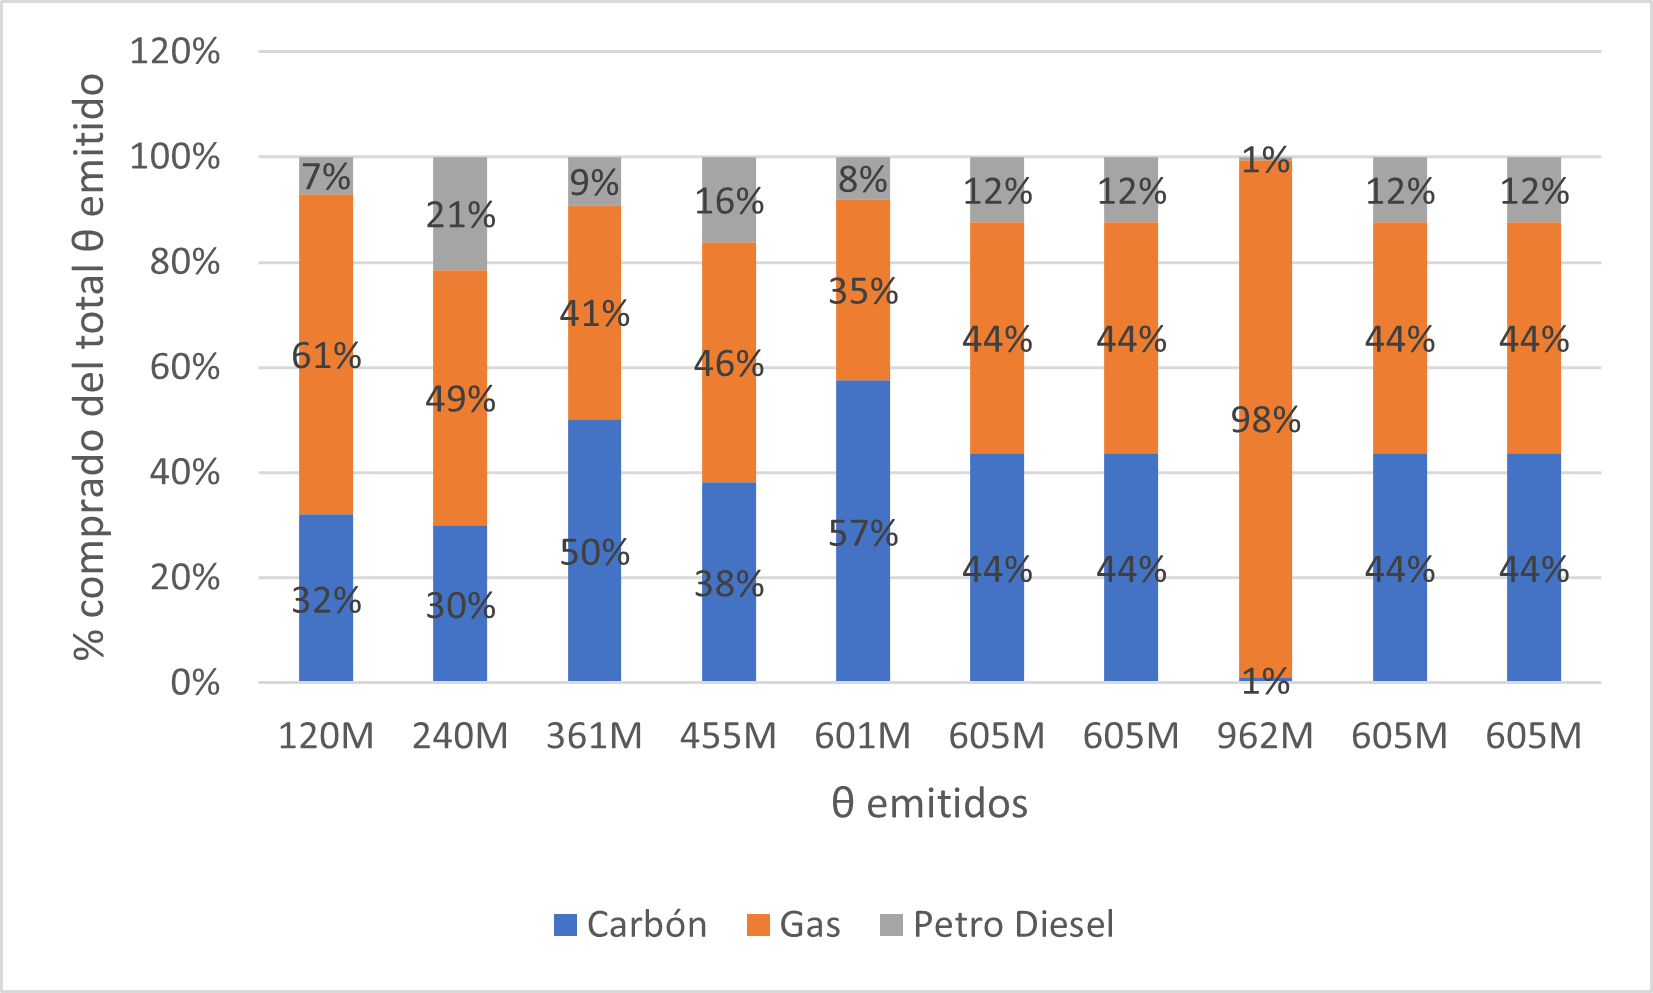
\includegraphics[width=\textwidth]{docs/DocumentoMemoria/core/images/distribucion primera etapa.png}
    \caption{{\footnotesize Primera etapa y $P=80\%$}}
    \label{petapaPO}
  \end{minipage}
  \hfill
  \begin{minipage}[b]{0.49\textwidth}
    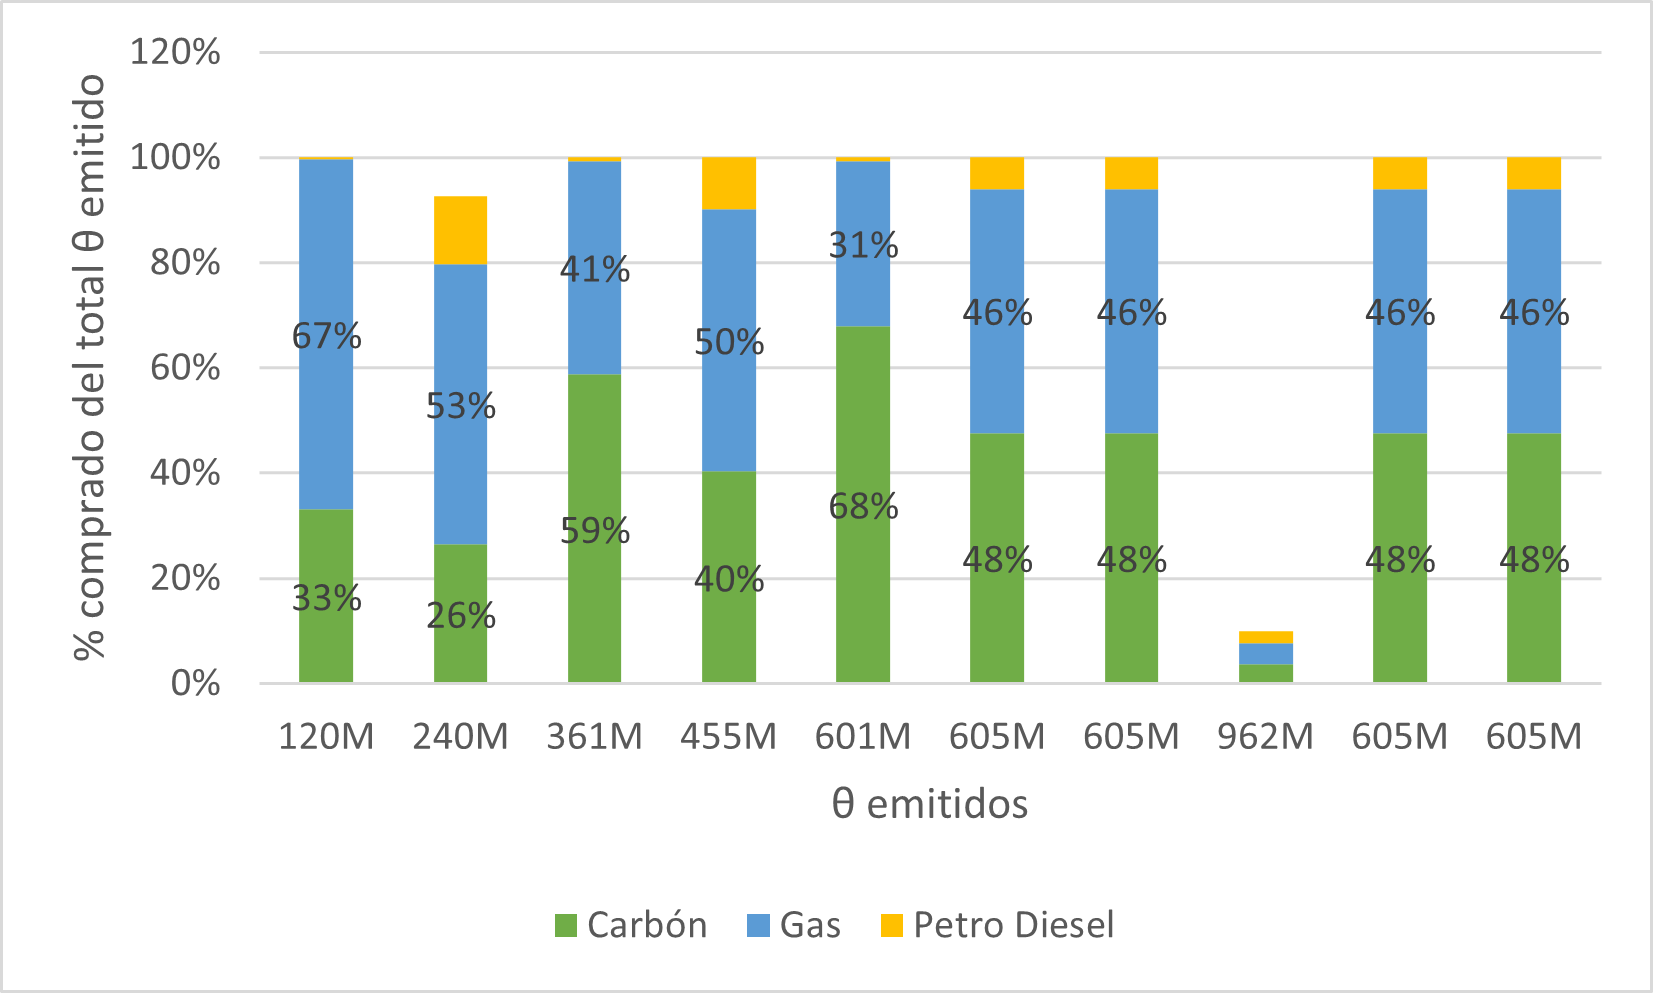
\includegraphics[width=\textwidth]{docs/DocumentoMemoria/core/images/distribucion segunda etapa.png}
    \caption{{\footnotesize Segunda etapa y $P=80\%$}}
    \label{setapaPO}
  \end{minipage}
\end{figure}

Para entender como este modelo afecta los permisos comprados por cada tecnología emisora de contaminante (al igual que el modelo original se consideran que estas son las empresas que usan Carbón, Gas y Petroleo como generador de electricidad), se grafican sus compras para cada cantidad de permisos emitidos (variando el CAP, manteniendo el rendimiento constante en $P=0.8$) en las figuras \ref{petapaPO} y \ref{setapaPO}.
\vspace{2.5mm}

En primer lugar, se grafica las distribuciones en la primera etapa, o sea, antes de que se revele el escenario de demanda energética en el futuro, en el cuál las empresas le compran los permisos al subastador. En segundo lugar, se grafica la nueva distribución para cada cantidad de permisos emitidos. Esta nueva distribución ocurre en la segunda etapa, donde las empresas forman un mercado de compra y venta de permisos entre ellas.
\vspace{2.5mm}

Por ejemplo, para un $CAP=100MtCO_2$, se emitieron 120 millones de permisos de contaminación. De los cuales el Gas compró un $61\%$ de esto, el Carbón un $32\%$ y el Petro Diesel un $7\%$. Luego, en la segunda etapa, estas tecnologías negociaron entre ellas (compras y ventas) y reajustaron su inversión en capacidad, llegando, finalmente, a que el GAS tiene un $67\%$ del total de permisos, el carbón un $33\%$ y el Petro Diesel vendió todos sus permisos. 
\vspace{2.5mm}

Estos resultados muestran que la dominancia (en cuanto a cantidad de permisos comprados) se mantiene estable entre etapas, siendo para casi todo presupuesto de carbono el Gas el mayor comprador. En adición a lo anterior, se ecuentra que para una emisión de 920 millones de permisos, existe una venta casi total de permisos. Esto no debería suceder ya que existe la restricción de condiciones de mercado \ref{rescom:2}, lo que puede significar que la alta no linealidad del modelo puede estar presentando errores para algunos valores o que existe la posibilidad de inclusión de recompra de permisos por parte del subastador, lo que permite disminuir las emisiones a pesar de existir una gran cantidad de permisos.
\vspace{2.5mm}

\begin{table}[H]
\begin{footnotesize}
    \centering
    \begin{tabular}{|l|l|l|l|l|l|l|l|l|l|l|}
    \hline
        $CAP$ & 100M & 200M & 300M & 400M & 500M & 600M & 700M & 800M & 900M & 1000M \\ \hline
        $\theta$  & 120M & 240M & 361M & 455M & 601M & 605M & 605M & 961M & 605M & 605M \\ \hline
        $\pi^d$  &  \$264.03   &  \$119.37   &  \$136.85   &  \$95.39   &  \$102.94   &  \$83.32   &  \$83.32   &  \$174.56   &  \$83.32   &  \$83.32   \\ \hline
    \end{tabular}
    \caption{{\footnotesize Precio de electricidad ($\pi^d$) por CAP y $P=80\%$}}
    \label{POpidporcap}
\end{footnotesize}
\end{table}

Una de las variables indirectas al modelo del subastador pero sobre la cual es importante estudiar el efecto de la reformulación del subastador es el precio de venta de electricidad que las empresas le cobran a las personas en el periodo 2018-2050. Su estudio puede entregar información valiosa sobre el bienestar social que estos nuevos modelos produzcan.
\vspace{2.5mm}

En el Cuadro \ref{POpidporcap} se encuentran los precios de electricidad $\pi^d$ ofrecido por las empresas generadoras de electricidad en el año 2018 (primera etapa) para todos los CAP y sus permisos emitidos resultantes. Los resultados muestran que a menores CAP resultan en menore precios de electricidad, a excepción del $CAP= 800MtCO_2$, en el cuál el precio es el segundo mayor de la tabla. Esto puede deberse a que, según lo mostrado en la Figura \ref{setapaPO}, las empresas generadoras contaminadoras, venden todos sus permisos en la segunda etapa, entonces, estas suben sus precios de venta de electricidad en la primera etapa.
\vspace{2.5mm}

\begin{figure}[H]
\centering
\resizebox{14cm}{10cm}{%
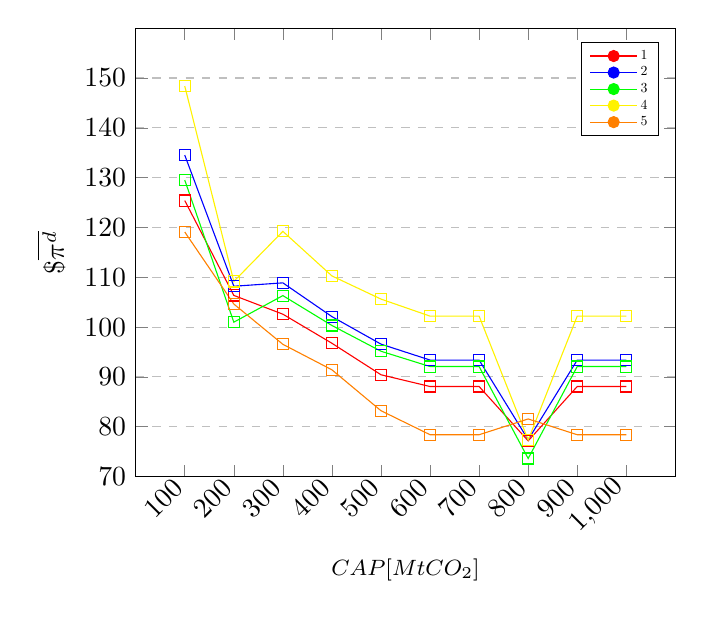
\begin{tikzpicture}
\centering
\begin{axis}[legend style={nodes={scale=0.5, transform shape}}, 
        legend image post style={mark=*},
    xlabel={{\footnotesize $CAP[MtCO_2]$}},
    xticklabel style = {rotate=45,anchor=east},
    ylabel={$\$ \overline{\pi^d}$},
    xmin=0, xmax=1100,
    ymin=70, ymax=160,
    xtick={100,200,300,400,500,600,700,800,900,1000},
    ytick={70,80,90,100,110,120,130,140,150},
    legend pos=north east,
    ymajorgrids=true,
    grid style=dashed,
]

\addplot[
    color=red,
    mark=square,
    ]
    coordinates {
    (100,125.4)(200,106.36)(300,102.59)(400,96.75)(500,90.43)(600,88.07)(700,88.07)(800,77.16)(900,88.07)(1000,88.07)
    };

\addplot[
    color=blue,
    mark=square,
    ]
    coordinates {(100,134.52)(200,108.2)(300,108.88)(400,102.1)(500,96.58)(600,93.38)(700,93.38)(800,77.39)(900,93.38)(1000,93.38)
    };
\addplot[
    color=green,
    mark=square,
    ]
    coordinates {
    (100,129.51)(200,100.99)(300,106.32)(400,100.32)(500,95.15)(600,92.08)(700,92.08)(800,73.62)(900,92.08)(1000,92.08)

    };
\addplot[
    color=yellow,
    mark=square,
    ]
    coordinates {
    (100,148.38)(200,109.17)(300,119.22)(400,110.27)(500,105.62)(600,102.2)(700,102.2)(800,77.33)(900,102.2)(1000,102.2)
    }; 
\addplot[
    color=orange,
    mark=square,
    ]
    coordinates {
    (100,119.09)(200,104.63)(300,96.54)(400,91.42)(500,83.21)(600,78.39)(700,78.39)(800,81.56)(900,78.39)(1000,78.39)
    };
    \legend{1,2,3,4,5}  
\end{axis}

\end{tikzpicture}
}

\caption{{\footnotesize Promedio de precios de electricidad (2019-2050)  por escenario}}
\label{rendcap}
\end{figure}

\begin{figure}[H]
\centering
\resizebox{13cm}{10cm}{%
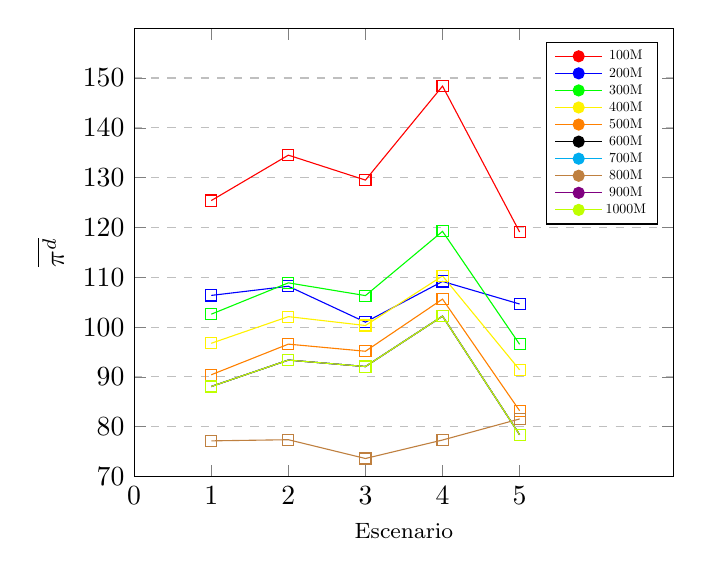
\begin{tikzpicture}
\centering
\begin{axis}[legend style={nodes={scale=0.5, transform shape}}, 
        legend image post style={mark=*},
    xlabel={{\footnotesize Escenario}},
    ylabel={$\overline{\pi^d}$},
    xmin=0, xmax=7,
    ymin=70, ymax=160,
    xtick={0,1,2,3,4,5},
    ytick={70,80,90,100,110,120,130,140,150},
    legend pos=north east,
    ymajorgrids=true,
    grid style=dashed,
]

\addplot[
    color=red,
    mark=square,
    ]
    coordinates {
    (1,125.4)(2,134.52)(3,129.51)(4,148.38)(5,119.09)
    };

\addplot[
    color=blue,
    mark=square,
    ]
    coordinates {(1,106.36)(2,108.2)(3,100.99)(4,109.17)(5,104.63)
    };
\addplot[
    color=green,
    mark=square,
    ]
    coordinates {
    (1,102.59)(2,108.88)(3,106.32)(4,119.22)(5,96.54)
    };
\addplot[
    color=yellow,
    mark=square,
    ]
    coordinates {
    (1,96.75)(2,102.1)(3,100.32)(4,110.27)(5,91.42)
    }; 
\addplot[
    color=orange,
    mark=square,
    ]
    coordinates {
    (1,90.43)(2,96.58)(3,95.15)(4,105.62)(5,83.21)
    };
\addplot[
    color=black,
    mark=square,
    ]
    coordinates {
    (1,88.07)(2,93.38)(3,92.08)(4,102.2)(5,78.39)
    };
\addplot[
    color=cyan,
    mark=square,
    ]
    coordinates {
    (1,88.07)(2,93.38)(3,92.08)(4,102.2)(5,78.39)
    };
\addplot[
    color=brown,
    mark=square,
    ]
    coordinates {
    (1,77.16)(2,77.39)(3,73.62)(4,77.33)(5,81.56)
    };
\addplot[
    color=violet,
    mark=square,
    ]
    coordinates {
    (1,88.07)(2,93.38)(3,92.08)(4,102.2)(5,78.39)
    };
\addplot[
    color=lime,
    mark=square,
    ]
    coordinates {
   (1,88.07)(2,93.38)(3,92.08)(4,102.2)(5,78.39)
    };
    \legend{100M, 200M,300M,400M,500M,600M,700M,800M,900M,1000M}

\end{axis}
\end{tikzpicture}
}
\caption{{\footnotesize Promedio de precios de electricidad (2019-2050)  por escenario}}
\label{rendcap}
\end{figure}




\section{Modelo de Bienestar Social con tasa cuadrada}

Este modelo, explicado en el capítulo \ref{tasacuadrada}, es resuelto como un único MCP de problema de equilibrio:
\vspace{2.5mm}

\textbf{MCP productor}

Se repite el MCP del productor presente en el capítulo anterior \ref{resultadosprofit}.

\textbf{MCP condiciones de mercado}

Al igual que el productor, este es el mismo MCP de las condiciones de mercado presente en el capítulo \ref{resultadosprofit}.

\textbf{MCP subastador}

\begin{tiny}
\begin{align}
    0 \leq \theta \perp - \pi^a + c(-2\theta + 2\hat{\theta})\frac{(2-2d-2(\frac{\theta - \hat{\theta}}{\hat{\theta}})^2)}{\hat{\theta}^2} - \eta \pi^a + c\eta((-2\theta + 2\hat{\theta})\frac{(2-2d-2(\frac{\theta - \hat{\theta}}{\hat{\theta}})^2)}{\hat{\theta}^2}) - \mu(\frac{-2\theta + 2\hat{\theta}}{\hat{\theta}^2}) - \lambda(\frac{2\theta-2\hat{\theta}}{\hat{\theta}^2}) \geq 0
\end{align}
\end{tiny}

\begin{footnotesize}
\begin{align}
    0 \leq \mu \perp 1 - \frac{(\theta-\hat{\theta})^2}{\hat{\theta}^2} - d  \geq 0\\
    0 \leq \lambda \perp \frac{(\theta-\hat{\theta})^2}{\hat{\theta}^2 }+ d \geq 0 \\
    0 \leq \eta \perp \theta \pi^a - c(1-\frac{(\theta - \hat{\theta})^2}{\hat{\theta}^2}-d)^2 \geq 0
\end{align}
\end{footnotesize}

\subsection{Calibración del modelo}

\begin{table}[H]
    \centering
    \begin{tabular}{|l|l|l|l|l|l|}
    \hline
        c & $\pi^a$ & $\theta$ & $\pi^a$ original &  CAP& $\Delta \pi^a$    \\ \hline
         \$1,000,000  &  \$51.76  & 3.02E+08 &  \$315.83  & 1.00E+08 &  \$264.07   \\ \hline
         \$10,000,000  &  \$212.84  & 1.63E+08 &  \$315.83  & 1.00E+08 &  \$102.98   \\ \hline
         \$100,000,000  &  \$220.51  & 1.55E+08 &  \$315.83  & 1.00E+08 &  \$95.31   \\ \hline
         \$109,000,000  &  \$142.81  & 9.10E+07 &  \$315.83  & 1.00E+08 &  \$173.02   \\ \hline
         \$9,000,000,000  &  \$181.21  & 1.98E+08 &  \$315.83  & 1.00E+08 &  \$134.62   \\ \hline
         \$9,500,000,000  &  \$184.11  & 1.97E+08 &  \$315.83  & 1.00E+08 &  \$131.72   \\ \hline
         \$9,900,000,000  &  \$232.82  & 1.45E+08 &  \$315.83  & 1.00E+08 &  \$83.01   \\ \hline
         \$9,999,000,000  &  \$232.82  & 1.45E+08 &  \$315.83  & 1.00E+08 &  \$83.01   \\ \hline
         \$9,999,005,000  &  \$207.55  & 1.69E+08 &  \$315.83  & 1.00E+08 &  \$108.27   \\ \hline
         \$9,999,500,000  &  \$232.82  & 1.45E+08 &  \$315.83  & 1.00E+08 &  \$83.01   \\ \hline
         \$9,999,900,000  &  \$182.38  & 1.98E+08 &  \$315.83  & 1.00E+08 &  \$133.45   \\ \hline
         \$10,000,000,000  &  \$182.27  & 1.95E+08 &  \$315.83  & 1.00E+08 &  \$133.56   \\ \hline
         \$90,000,000,000  &  \$146.83  & 1.54E+08 &  \$315.83  & 1.00E+08 &  \$168.99   \\ \hline
         \$100,000,000,000  &  \$211.29  & 1.57E+08 &  \$315.83  & 1.00E+08 &  \$104.54   \\ \hline
         \$110,000,000,000  &  \$144.07  & 1.52E+08 &  \$315.83  & 1.00E+08 &  \$171.76   \\ \hline
         \$150,000,000,000  &  \$164.89  & 1.51E+08 &  \$315.83  & 1.00E+08 &  \$150.93   \\ \hline
         \$200,000,000,000  &  \$143.18  & 1.49E+08 &  \$315.83  & 1.00E+08 &  \$172.65   \\ \hline
    \end{tabular}
    \caption{{\footnotesize Precio de electricidad ($\pi^d$) por CAP}}
    \label{calibracioncuadrado}
\end{table}

Los resultados de la calibración, en el Cuadro \ref{calibracioncuadrado}, muestran que el costo marginal $c$ con el cuál se tiene una variable $\pi^a$ más cercana al original (manteniendo un CAP de $100MtCO_{2}e$), es con un $c=\$9,900,000,000$.

\subsection{Resultados}

Contrario al modelo anterior, en este modelo, el siguiente (Modelo con Precisión) y el original, el único parámetro que se varía para encontrar resultados es el presupuesto de carbono establecido por el gobierno (CAP). El rendimiento (P) se calcula con lso valores de las variables encontradas.
\vspace{2.5mm}

Según lo explicado en el Capítulo \ref{tasacuadrada}, el rendimiento se calcula de las siguiente forma: 
\vspace{2.5mm}

\begin{equation}
\begin{array}{rrclcl}
\displaystyle P = 1- (\frac{{\theta - \hat{\theta}}}{\hat{\theta}})^2 \\
\end{array}
\end{equation}

Considerando lo anterior, se tienen los siguientes resultados:

\begin{table}[H]
    \centering
    \begin{tabular}{|l|l|l|l|l|}
    \hline
        CAP & $\theta$ & Rend[P] & $\frac{\theta}{CAP}$  & $\pi^a$  \\ \hline
        100,000,000 & 144,944,410  & 0.798  & 1.449  &  \$232.82   \\ \hline
        200,000,000 & 289,888,820  & 0.798  & 1.449  &  \$141.56   \\ \hline
        300,000,000 & 434,833,230  & 0.798  & 1.449  &  \$103.33   \\ \hline
        400,000,000 & 579,777,640  & 0.798  & 1.449  &  \$-   \\ \hline
        500,000,000 & 653,754,577  & 0.905  & 1.308  &  \$37.27   \\ \hline
        600,000,000 & 619,939,821  & 0.999  & 1.033  &  \$40.43   \\ \hline
        700,000,000 & 661,258,561  & 0.997  & 0.945  &  \$36.42   \\ \hline
        800,000,000 & 610,913,181  & 0.944  & 0.764  &  \$31.28   \\ \hline
        900,000,000 & 609,127,279  & 0.896  & 0.677  &  \$31.21   \\ \hline
        1,000,000,000 & 698,676,376  & 0.909  & 0.699  &  \$30.00   \\ \hline
    \end{tabular}
    \caption{{\footnotesize Resultados modelo tasa al cuadrado}}
    \label{resultadostasacuadrada}
\end{table}

\begin{figure}[H]
\centering
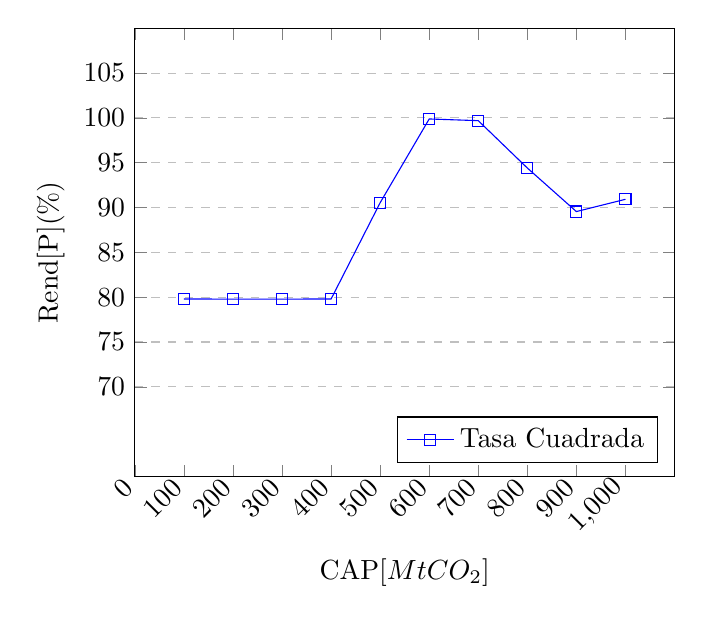
\begin{tikzpicture}
\begin{axis}[
    xlabel={CAP[$MtCO_2$]},
    ylabel={Rend[P](\%)},
    xmin=0, xmax=1100,
    ymin=60, ymax=110,
    xtick={0,100,200,300,400,500,600,700,800,900,1000},
    xticklabel style = {rotate=45,anchor=east},
    ytick={70,75,80,85,90,95,100,105},
    legend pos=south east,
    ymajorgrids=true,
    grid style=dashed,
]

\addplot[
    color=blue,
    mark=square,
    ]
    coordinates {
    (100,79.8)(200,79.79)(300,79.79)(400,79.8)(500,90.54)(600,99.88)(700,99.69)(800,94.41)(900,89.55)(1000,90.92)
    };
    \legend{Tasa Cuadrada}
    
\end{axis}
\end{tikzpicture}
\caption{{\footnotesize Efecto del CAP sobre P}}
\label{rendcap}
\end{figure}

\begin{figure}[H]
\centering
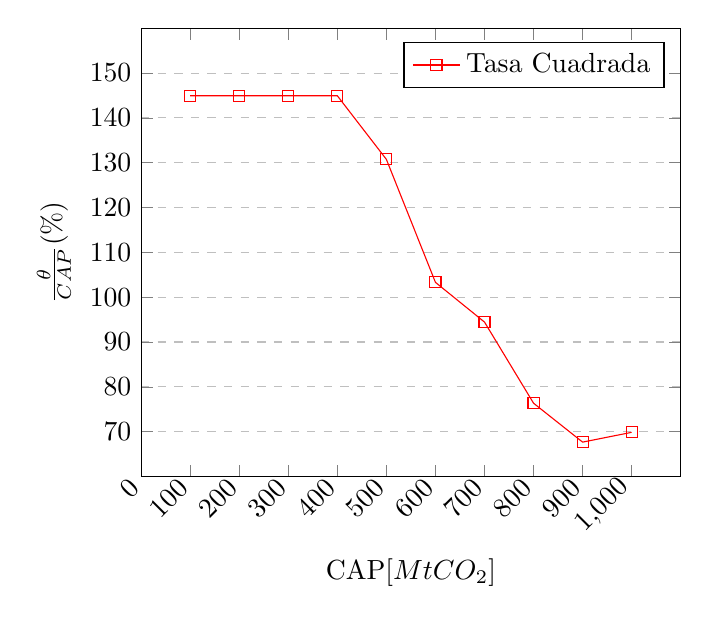
\begin{tikzpicture}
\begin{axis}[
    xlabel={CAP[$MtCO_2$]},
    ylabel={$\frac{\theta}{CAP}(\%)$},
    xmin=0, xmax=1100,
    ymin=60, ymax=160,
    xtick={0,100,200,300,400,500,600,700,800,900,1000},
    xticklabel style = {rotate=45,anchor=east},
    ytick={70,80,90,100,110,120,130,140,150},
    legend pos=north east,
    ymajorgrids=true,
    grid style=dashed,
]

\addplot[
    color=red,
    mark=square,
    ]
    coordinates {
    (100,144.94)(200,144.94)(300,144.94)(400,144.94)(500,130.75)(600,103.32)(700,94.46)(800,76.36)(900,67.68)(1000,69.86)
    };
    \legend{Tasa Cuadrada}
    
\end{axis}
\end{tikzpicture}
\caption{{\footnotesize Efecto del CAP sobre $\frac{\theta}{CAP}$}}
\label{rendcap}
\end{figure}

\begin{figure}[H]
  \centering
  \begin{minipage}[b]{0.49\textwidth}
    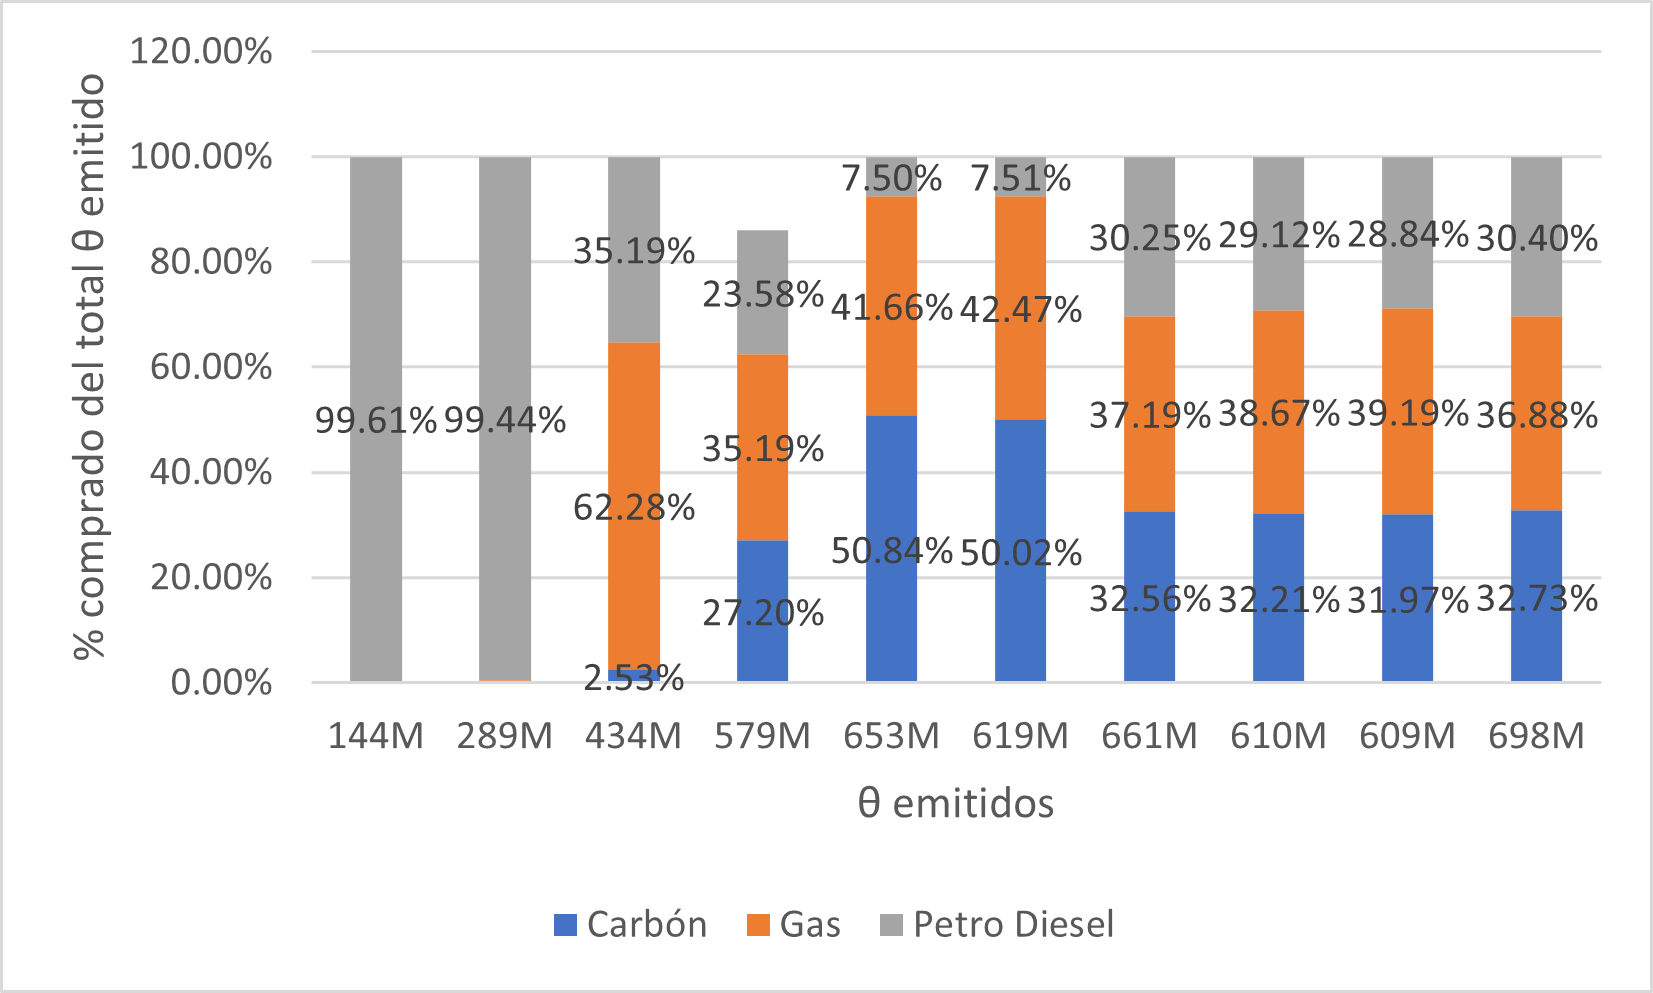
\includegraphics[width=\textwidth]{docs/DocumentoMemoria/core/images/distr primera etapa tasa cuadrada.png}
    \caption{{\footnotesize Distribución Primera Etapa}}
  \end{minipage}
  \hfill
  \begin{minipage}[b]{0.49\textwidth}
    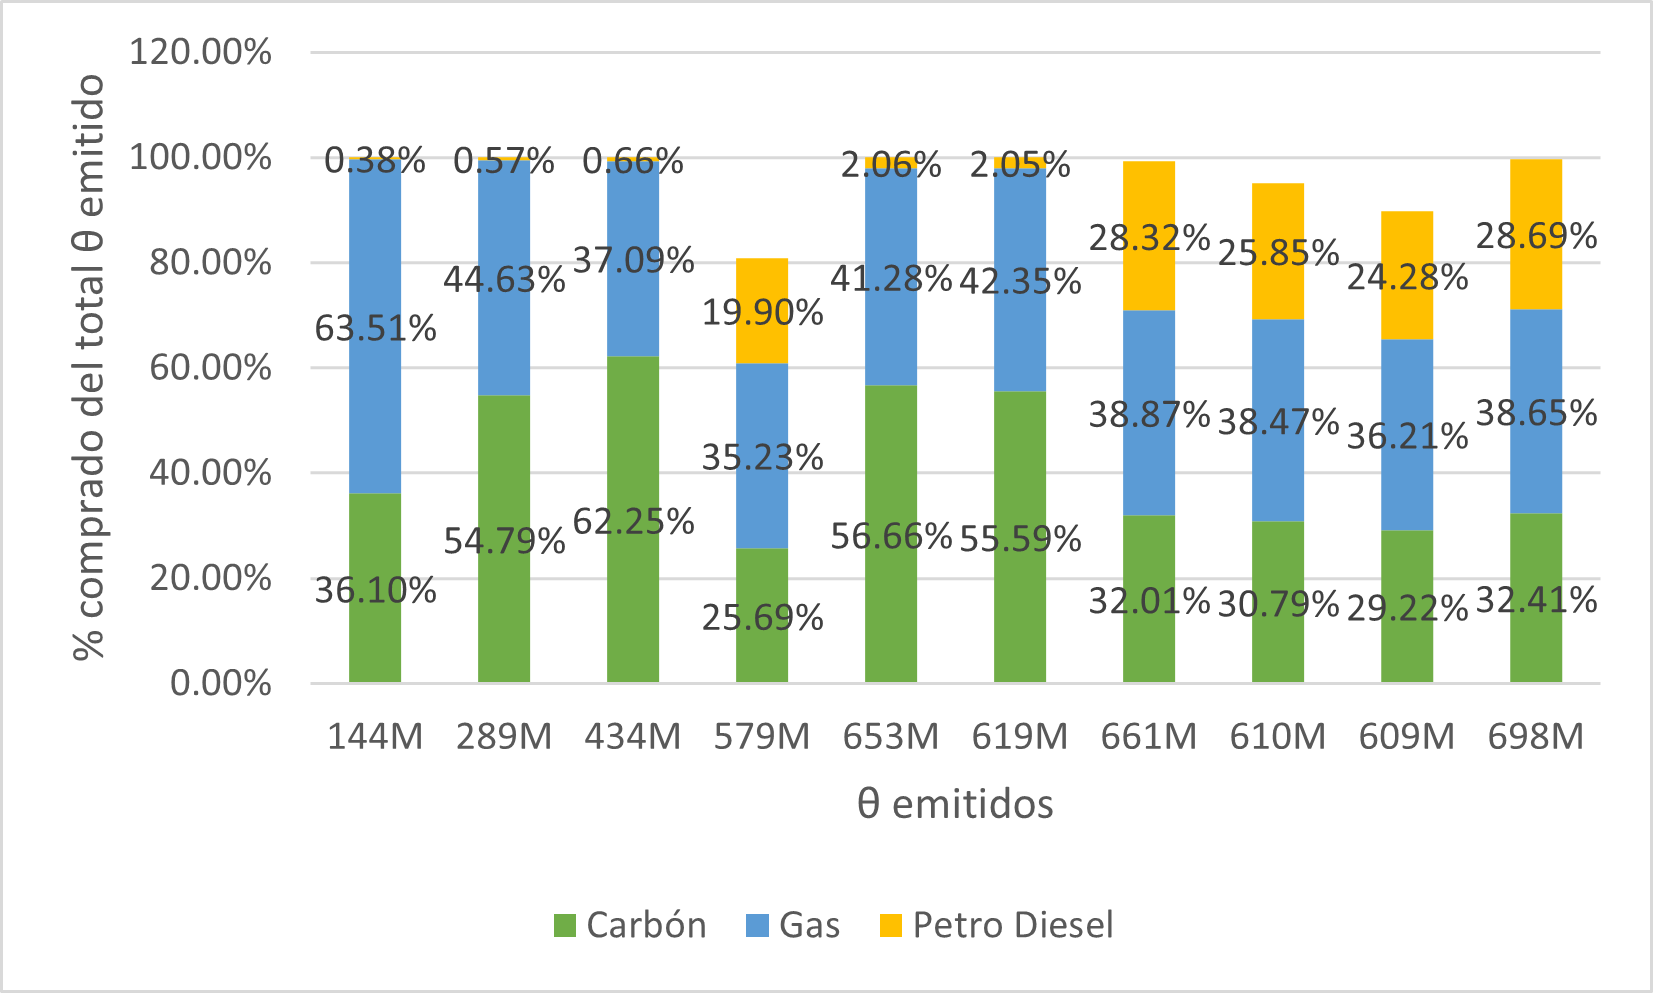
\includegraphics[width=\textwidth]{docs/DocumentoMemoria/core/images/distr segunda etapa tasa cuadrada.png}
    \caption{{\footnotesize Distribución Segunda Etapa}}
  \end{minipage}
\end{figure}

\begin{table}[H]
\begin{footnotesize}
    \centering
    \begin{tabular}{|l|l|l|l|l|l|l|l|l|l|l|}
    \hline
        CAP[$MtCO_2$] & 100 & 200 & 300 & 400 & 500 & 600 & 700 & 800 & 900 & 1000 \\ \hline
       $\theta$[Millones]  & 145  & 290  & 435  & 580  & 654  & 620  & 661  & 611  & 609  & 699  \\ \hline
        $\pi^d$  &  \$232.54   &  \$155.49   &  \$123.21   &  \$93.90   &  \$87.48   &  \$90.44   &  \$105.74   &  \$95.05   &  \$93.38   &  \$94.53   \\ \hline
    \end{tabular}
    \caption{{\footnotesize Precio de electricidad ($\pi^d$) en el año 2018 por CAP }}
    \label{TCpidporcap}
\end{footnotesize}
\end{table}

\begin{figure}[H]
\centering
\resizebox{13cm}{10cm}{%
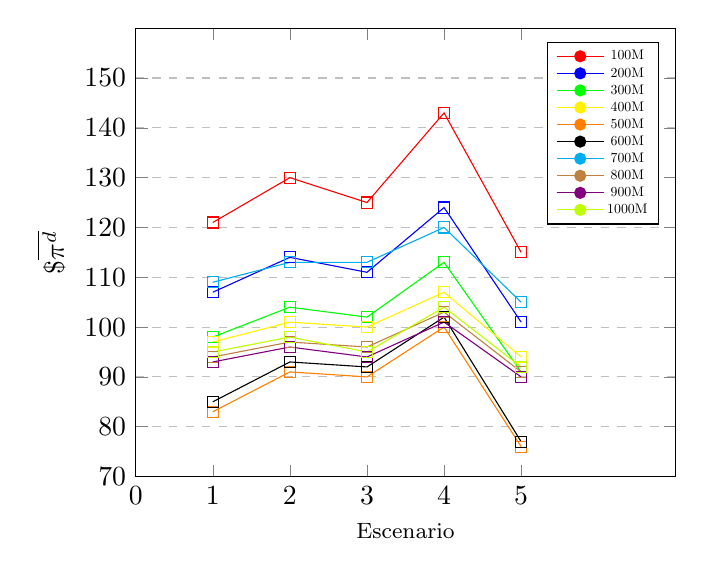
\begin{tikzpicture}
\centering
\begin{axis}[legend style={nodes={scale=0.5, transform shape}}, 
        legend image post style={mark=*},
    xlabel={{\footnotesize Escenario}},
    ylabel={$\$ \overline{\pi^d}$},
    xmin=0, xmax=7,
    ymin=70, ymax=160,
    xtick={0,1,2,3,4,5},
    ytick={70,80,90,100,110,120,130,140,150},
    legend pos=north east,
    ymajorgrids=true,
    grid style=dashed,
]

\addplot[
    color=red,
    mark=square,
    ]
    coordinates {
    (1,121)(2,130)(3,125)(4,143)(5,115)
    };

\addplot[
    color=blue,
    mark=square,
    ]
    coordinates {(1,107)(2,114)(3,111)(4,124)(5,101)
    };
\addplot[
    color=green,
    mark=square,
    ]
    coordinates {
    (1,98)(2,104)(3,102)(4,113)(5,91)
    };
\addplot[
    color=yellow,
    mark=square,
    ]
    coordinates {
    (1,97)(2,101)(3,100)(4,107)(5,94)
    }; 
\addplot[
    color=orange,
    mark=square,
    ]
    coordinates {
    (1,83)(2,91)(3,90)(4,100)(5,76)
    };
\addplot[
    color=black,
    mark=square,
    ]
    coordinates {
    (1,85)(2,93)(3,92)(4,102)(5,77)
    };
\addplot[
    color=cyan,
    mark=square,
    ]
    coordinates {
    (1,109)(2,113)(3,113)(4,120)(5,105)
    };
\addplot[
    color=brown,
    mark=square,
    ]
    coordinates {
    (1,94)(2,97)(3,96)(4,103)(5,91)
    };
\addplot[
    color=violet,
    mark=square,
    ]
    coordinates {
    (1,93)(2,96)(3,94)(4,101)(5,90)
    };
\addplot[
    color=lime,
    mark=square,
    ]
    coordinates {
   (1,95)(2,98)(3,95)(4,104)(5,92)
    };
    \legend{100M, 200M,300M,400M,500M,600M,700M,800M,900M,1000M}

\end{axis}
\end{tikzpicture}
}
\caption{{\footnotesize Precios de electricidad (2019-2050)  por escenario}}
\label{TCrendcap}
\end{figure}


\section{Modelo de Bienestar Social con precisión}

Esta versión, utilizando el concepto de precisión, se resuelve, al igual que los dos anteriores, como un problema de equilibrio en formato MCP:
\vspace{2.5mm}

\textbf{MCP productor}

Se repite el MCP del productor presente en el capítulo \ref{resultadosprofit}.

\textbf{MCP condiciones de mercado}

Al igual que del productor, este es el mismo MCP de la condiciones de mercado presente en el capítulo \ref{resultadosprofit}.

\textbf{MCP subastador}

\begin{footnotesize}
\begin{align}
    0 \leq \theta \perp -\pi^a   - \eta\pi^a  + \lambda -  \delta \geq 0\\
   0 \leq r \perp 2c\frac{(-1+d+\frac{r}{\hat{\theta}})}{\hat{\theta}} + 2c\eta \frac{(-1+d+\frac{r}{\hat{\theta}})}{\hat{\theta}} - \lambda - \delta  \geq 0\\
0 \leq \eta \perp \theta \pi^a - c(1-\frac{r}{\hat{\theta}}-d)^2 \geq 0 \\
0 \leq \lambda \perp r - \theta + \hat{\theta} \geq 0 \\
0 \leq \delta \perp r + \theta - \hat{\theta} \geq 0\\
0 \leq \mu \perp 1-\frac{r}{\hat{\theta}}-d \geq 0\\
0 \leq\chi \perp \frac{r}{\hat{\theta}} + d \geq 0 
\end{align}
\end{footnotesize}

\subsection{Calibración del modelo}

\begin{table}[H]
    \centering
    \begin{tabular}{|l|l|l|l|l|l|}
    \hline
          c & $\pi^a$ & $\theta$ & $\pi^a$ original &  CAP & $\Delta \pi^a$   \\ \hline
         \$50  &  \$244.34  & 1.20E+08 &  \$315.83  & 1.00E+08 & 71.482  \\ \hline
         \$500  &  \$219.60  & 1.20E+08 &  \$315.83  & 1.00E+08 & 96.229  \\ \hline
         \$5,000  &  \$209.14  & 1.20E+08 &  \$315.83  & 1.00E+08 & 106.689  \\ \hline
         \$50,000  &  \$219.41  & 1.20E+08 &  \$315.83  & 1.00E+08 & 96.415  \\ \hline
         \$500,000  &  \$213.10  & 1.20E+08 &  \$315.83  & 1.00E+08 & 102.723  \\ \hline
         \$3,000,000  &  \$205.23  & 1.20E+08 &  \$315.83  & 1.00E+08 & 110.593  \\ \hline
         \$3,500,000  &  \$198.96  & 1.20E+08 &  \$315.83  & 1.00E+08 & 116.864  \\ \hline
         \$3,900,000  &  \$218.76  & 1.20E+08 &  \$315.83  & 1.00E+08 & 97.067  \\ \hline
         \$4,000,000  &  \$270.13  & 1.20E+08 &  \$315.83  & 1.00E+08 & 45.699  \\ \hline
         \$4,000,001  &  \$194.42  & 1.20E+08 &  \$315.83  & 1.00E+08 & 121.405  \\ \hline
         \$4,000,005  &  \$270.13  & 1.20E+08 &  \$315.83  & 1.00E+08 & 45.699  \\ \hline
         \$5,000,000  &  \$270.13  & 1.20E+08 &  \$315.83  & 1.00E+08 & 45.699  \\ \hline
         \$6,000,000  &  \$212.54  & 1.20E+08 &  \$315.83  & 1.00E+08 & 103.286  \\ \hline
         \$50,000,000  &  \$270.13  & 1.20E+08 &  \$315.83  & 1.00E+08 & 45.699  \\ \hline
         \$500,000,000  &  \$270.13  & 1.20E+08 &  \$315.83  & 1.00E+08 & 45.699  \\ \hline
         \$5,000,000,000  &  \$270.13  & 1.20E+08 &  \$315.83  & 1.00E+08 & 45.699  \\ \hline
         \$50,000,000,000  &  \$237.74  & 1.20E+08 &  \$315.83  & 1.00E+08 & 78.09  \\ \hline
    \end{tabular}
    \caption{{\footnotesize Calibración modelo Precisión }}
    \label{calibracionprecision}
\end{table}

Los resultados de la calibración, en el Cuadro \ref{calibracionprecision}, muestran que el costo marginal $c$ con el cuál se tiene una variable $\pi^a$ más cercana al original (manteniendo un CAP de $100MtCO_{2}e$), es con un $c=\$4,000,000$.

\subsection{Resultados}

Según lo explicado en el Capítulo \ref{modeloconprecision}, el rendimiento se calcula de las siguiente forma: 
\vspace{2.5mm}

\begin{equation}
\begin{array}{rrclcl}
\displaystyle P = 1- \frac{r}{\hat{\theta}} \\
\end{array}
\end{equation}

Considerando lo anterior, se tienen los siguientes resultados:

\begin{table}[H]
    \centering
    \begin{tabular}{|l|l|l|l|l|}
    \hline
        CAP & $\theta$ & Rend[P] & $\frac{\theta}{CAP}$  & $\pi^a$ \\ \hline
        100,000,000 & 120,200,000  & 0.798  & 1.202  &  \$270.13   \\ \hline
        200,000,000 & 240,400,000  & 0.798  & 1.202  &  \$155.15   \\ \hline
        300,000,000 & 354,508,234  & 0.798  & 1.182  &  \$39.07   \\ \hline
        400,000,000 & 435,648,945  & 0.798  & 1.089  &  \$33.93   \\ \hline
        500,000,000 & 590,042,475  & 0.798  & 1.180  &  \$38.83   \\ \hline
        600,000,000 & 721,200,000  & 0.798  & 1.202  &  \$39.20   \\ \hline
        700,000,000 & 673,836,382  & 0.798  & 0.963  &  \$35.74   \\ \hline
        800,000,000 & 757,247,245  & 0.798  & 0.947  &  \$35.74   \\ \hline
        900,000,000 & 851,903,151  & 0.798  & 0.947  &  \$35.74   \\ \hline
        1,000,000,000 & 947,173,004  & 0.798  & 0.947  &  \$35.74   \\ \hline
    \end{tabular}
    \caption{{\footnotesize Resultados modelo Precisión}}
    \label{resultadosprecision}
\end{table}

\begin{figure}[H]
\centering
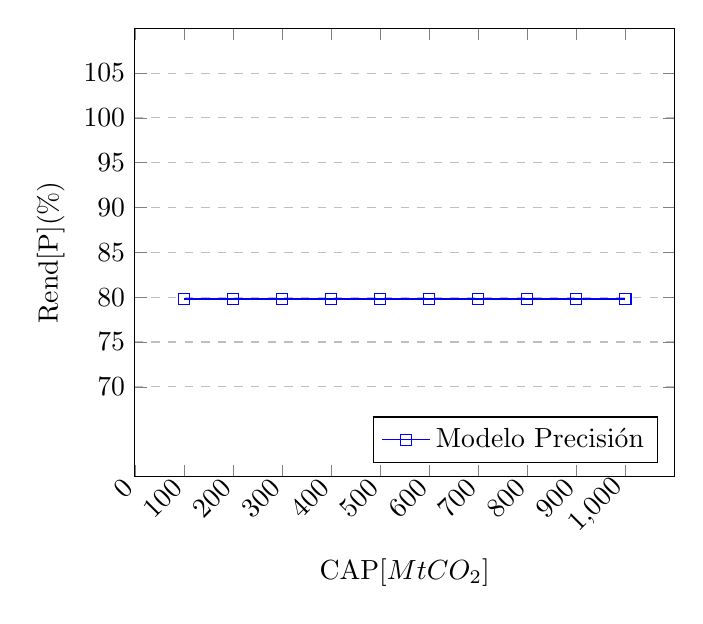
\begin{tikzpicture}
\begin{axis}[
    xlabel={CAP[$MtCO_2$]},
    ylabel={Rend[P](\%)},
    xmin=0, xmax=1100,
    ymin=60, ymax=110,
    xtick={0,100,200,300,400,500,600,700,800,900,1000},
    xticklabel style = {rotate=45,anchor=east},
    ytick={70,75,80,85,90,95,100,105},
    legend pos=south east,
    ymajorgrids=true,
    grid style=dashed,
]

\addplot[
    color=blue,
    mark=square,
    ]
    coordinates {
    (100,79.8)(200,79.8)(300,79.8)(400,79.8)(500,79.8)(600,79.8)(700,79.8)(800,79.8)(900,79.8)(1000,79.8)
    };
    \legend{Modelo Precisión}
    
\end{axis}
\end{tikzpicture}
\caption{{\footnotesize Efecto del CAP sobre P}}
\label{rendcap}
\end{figure}

\begin{figure}[H]
\centering
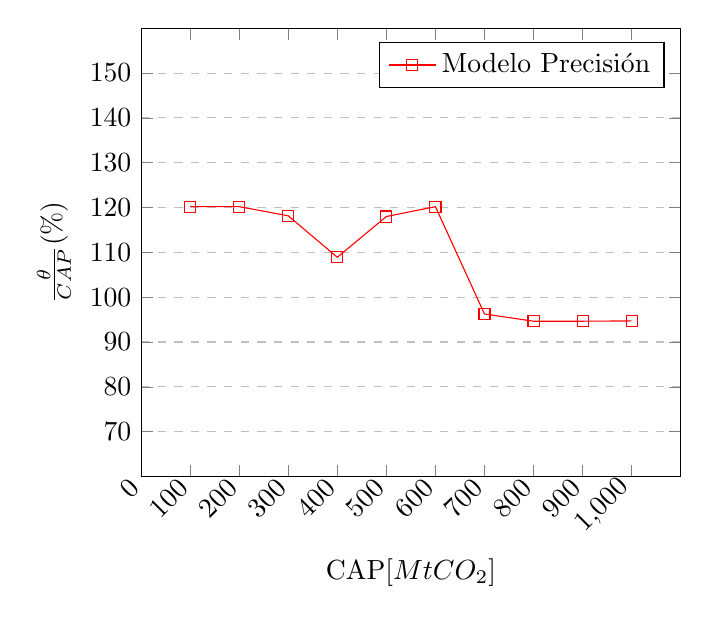
\begin{tikzpicture}
\begin{axis}[
    xlabel={CAP[$MtCO_2$]},
    ylabel={$\frac{\theta}{CAP}(\%)$},
    xmin=0, xmax=1100,
    ymin=60, ymax=160,
    xtick={0,100,200,300,400,500,600,700,800,900,1000},
    xticklabel style = {rotate=45,anchor=east},
    ytick={70,80,90,100,110,120,130,140,150},
    legend pos=north east,
    ymajorgrids=true,
    grid style=dashed,
]

\addplot[
    color=red,
    mark=square,
    ]
    coordinates {
    (100,120.2)(200,120.2)(300,118.16)(400,108.91)(500,118)(600,120.2)(700,96.26)(800,94.65)(900,94.65)(1000,94.71)
    };
    \legend{Modelo Precisión}
    
\end{axis}
\end{tikzpicture}
\caption{{\footnotesize Efecto del CAP sobre $\frac{\theta}{CAP}$}}
\label{rendcap}
\end{figure}

\begin{figure}[H]
  \centering
  \begin{minipage}[b]{0.49\textwidth}
    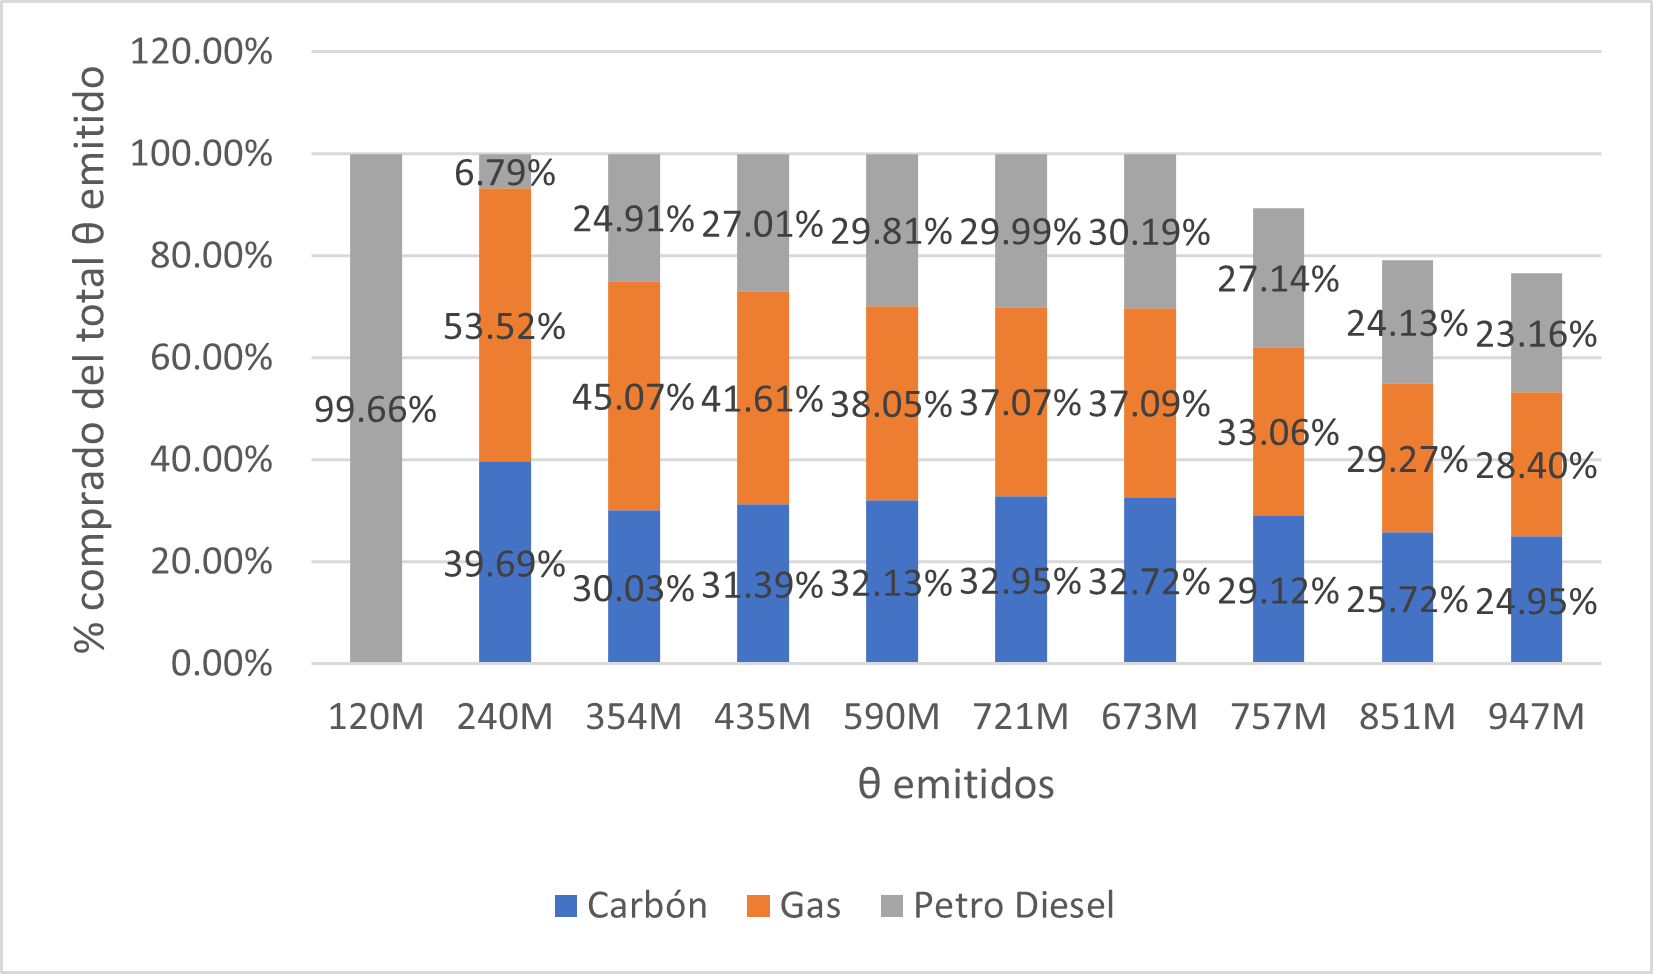
\includegraphics[width=\textwidth]{docs/DocumentoMemoria/core/images/distr primera etapa precision.png}
    \caption{{\footnotesize Distribución Primera Etapa}}
  \end{minipage}
  \hfill
  \begin{minipage}[b]{0.49\textwidth}
    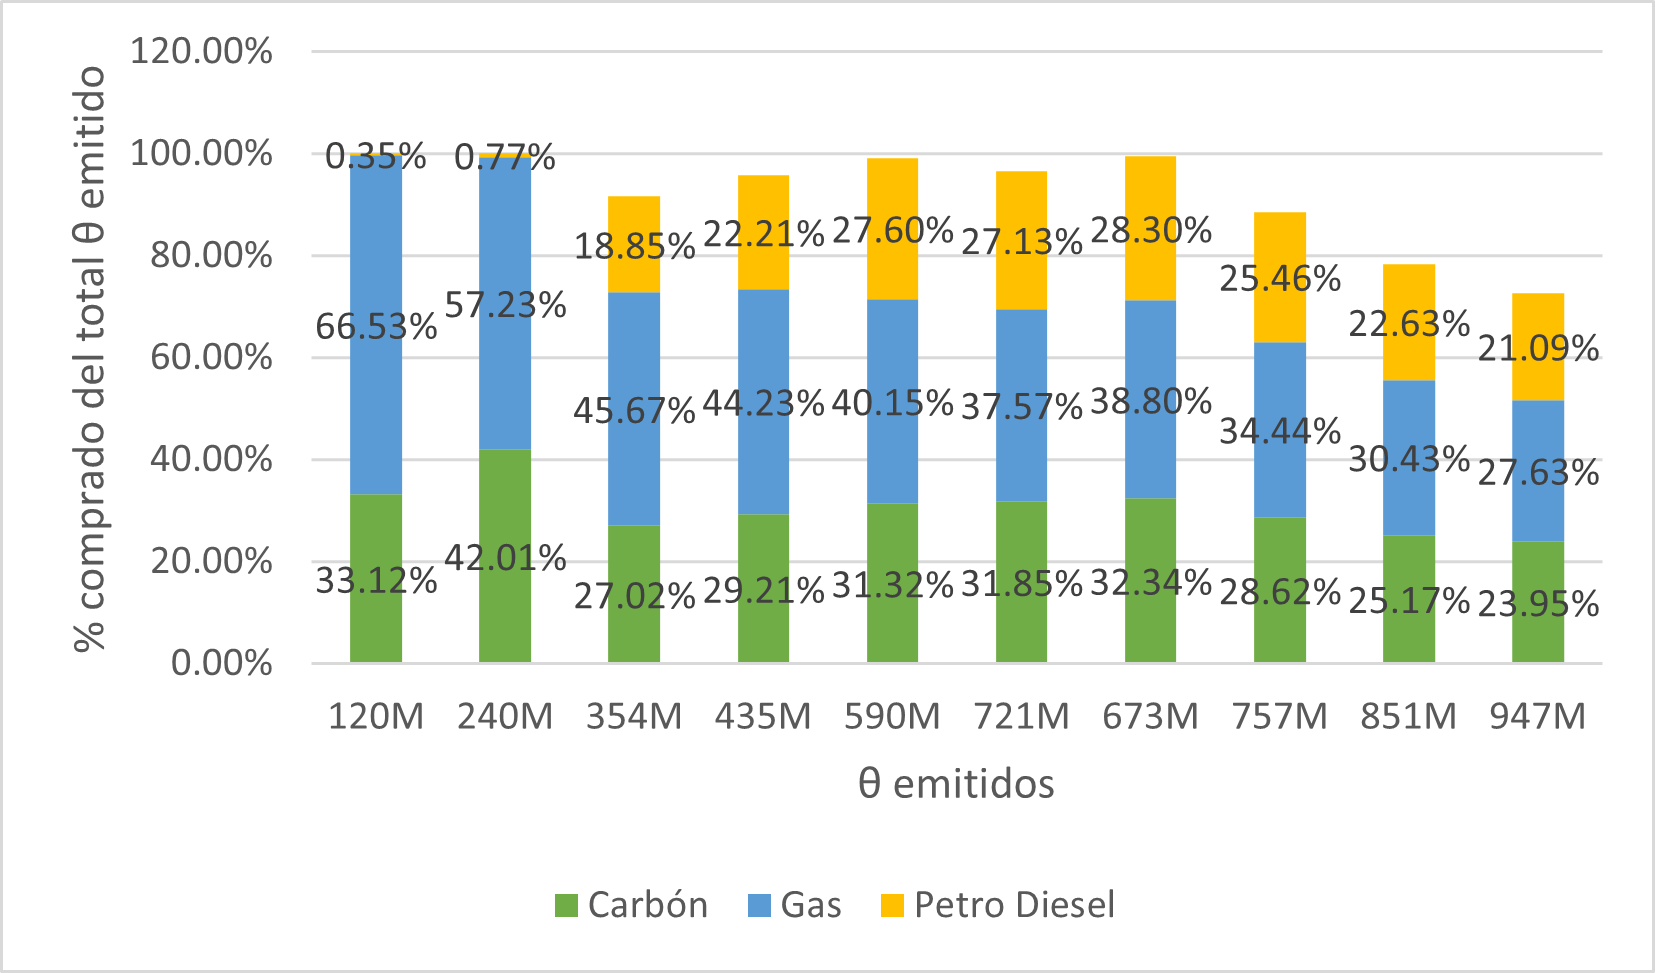
\includegraphics[width=\textwidth]{docs/DocumentoMemoria/core/images/distr segunda etapa precision.png}
    \caption{{\footnotesize Distribución Segunda Etapa}}
  \end{minipage}
\end{figure}

\begin{table}[H]
\begin{footnotesize}
    \centering
    \begin{tabular}{|l|l|l|l|l|l|l|l|l|l|l|}
    \hline
       CAP[$MtCO_2$] & 100 & 200 & 300 & 400 & 500 & 600 & 700 & 800 & 900 & 1000 \\ \hline
          $\theta$[Millones] & 120 & 240 & 355 & 436 & 590 & 721 & 674 & 757 & 852 & 947 \\ \hline
    $\pi^d$  &  \$264.03   &  \$169.98   &  \$106.88   &  \$98.92   &  \$110.36   &  \$93.00   &  \$105.33   &  \$99.07   &  \$97.95   &  \$92.09   \\ \hline
    \end{tabular}
    \caption{{\footnotesize Precio de electricidad ($\pi^d$) en el año 2018 por CAP }}
    \label{Ppidporcap}
\end{footnotesize}
\end{table}

\begin{figure}[H]
\centering
\resizebox{13cm}{10cm}{%
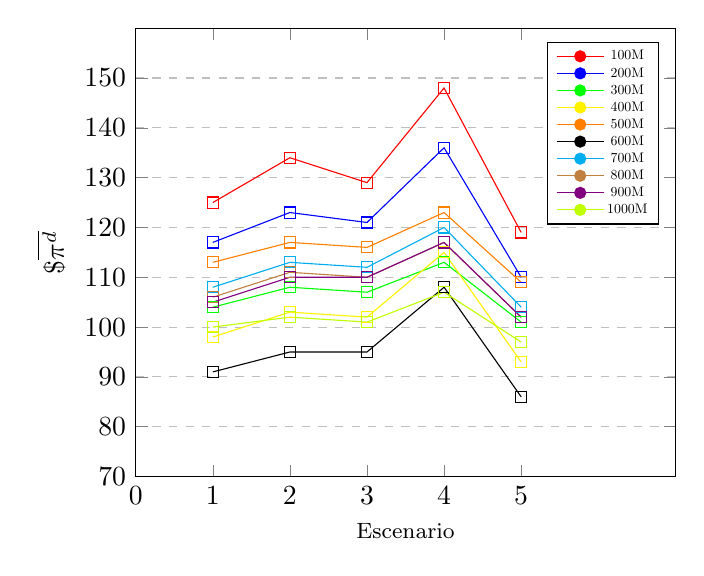
\begin{tikzpicture}
\centering
\begin{axis}[legend style={nodes={scale=0.5, transform shape}}, 
        legend image post style={mark=*},
    xlabel={{\footnotesize Escenario}},
    ylabel={$\$ \overline{\pi^d}$},
    xmin=0, xmax=7,
    ymin=70, ymax=160,
    xtick={0,1,2,3,4,5},
    ytick={70,80,90,100,110,120,130,140,150},
    legend pos=north east,
    ymajorgrids=true,
    grid style=dashed,
]

\addplot[
    color=red,
    mark=square,
    ]
    coordinates {
    (1,125)(2,134)(3,129)(4,148)(5,119)
    };

\addplot[
    color=blue,
    mark=square,
    ]
    coordinates {(1,117)(2,123)(3,121)(4,136)(5,110)
    };
\addplot[
    color=green,
    mark=square,
    ]
    coordinates {
    (1,104)(2,108)(3,107)(4,113)(5,101)
    };
\addplot[
    color=yellow,
    mark=square,
    ]
    coordinates {
    (1,98)(2,103)(3,102)(4,115)(5,93)
    }; 
\addplot[
    color=orange,
    mark=square,
    ]
    coordinates {
    (1,113)(2,117)(3,116)(4,123)(5,109)
    };
\addplot[
    color=black,
    mark=square,
    ]
    coordinates {
    (1,91)(2,95)(3,95)(4,108)(5,86)
    };
\addplot[
    color=cyan,
    mark=square,
    ]
    coordinates {
    (1,108)(2,113)(3,112)(4,120)(5,104)
    };
\addplot[
    color=brown,
    mark=square,
    ]
    coordinates {
    (1,106)(2,111)(3,110)(4,117)(5,102)
    };
\addplot[
    color=violet,
    mark=square,
    ]
    coordinates {
    (1,105)(2,110)(3,110)(4,117)(5,102)
    };
\addplot[
    color=lime,
    mark=square,
    ]
    coordinates {
   (1,100)(2,102)(3,101)(4,107)(5,97)
    };
    \legend{100M, 200M,300M,400M,500M,600M,700M,800M,900M,1000M}

\end{axis}
\end{tikzpicture}
}
\caption{{\footnotesize Precios de electricidad (2019-2050)  por escenario}}
\label{TCrendcap}
\end{figure}

\section{Comparación de Modelos}

\begin{figure}[H]
    \centering
    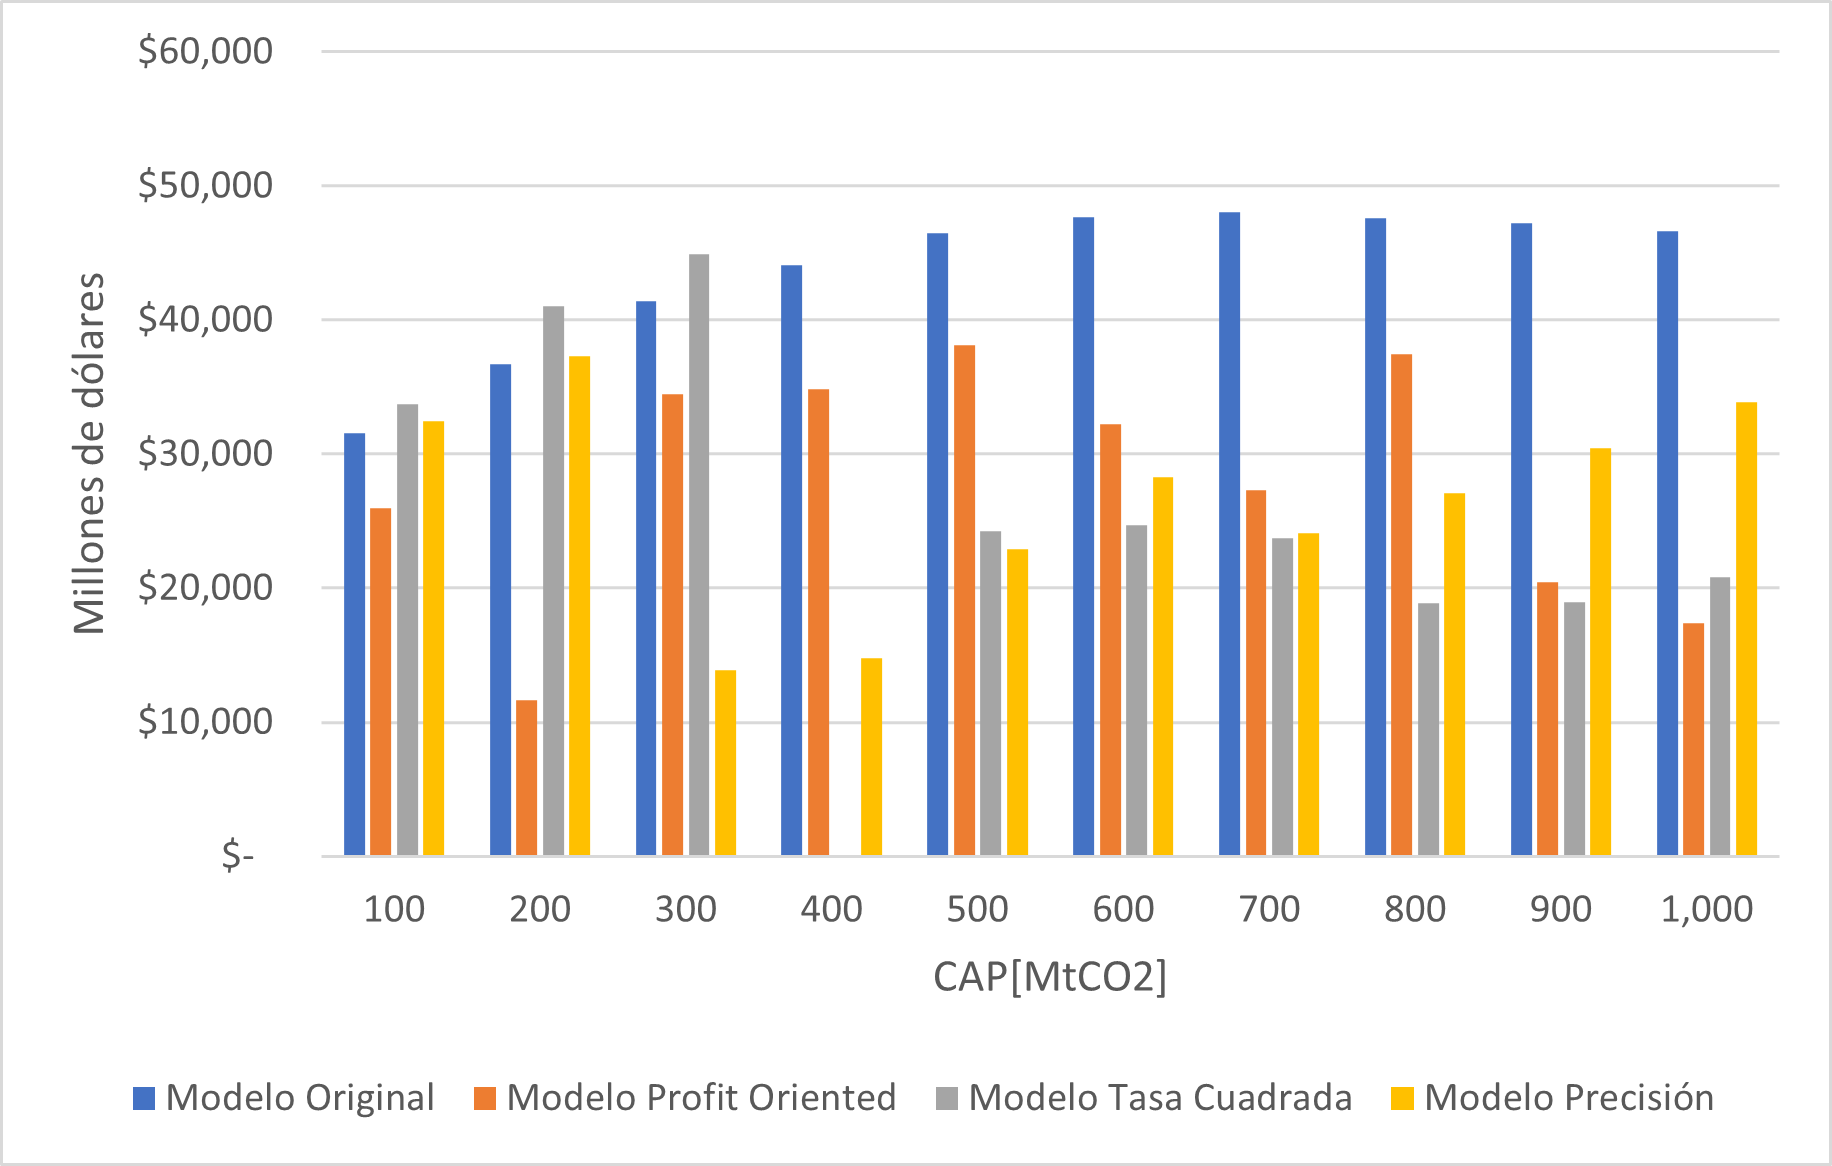
\includegraphics[width=12cm]{docs/DocumentoMemoria/core/images/utilidad de todos lo modelos.png}
    \caption{Utilidad del subastador por modelo }
    \label{utilidades}
\end{figure}


\begin{figure}[H]
\centering
\resizebox{12cm}{9cm}{%
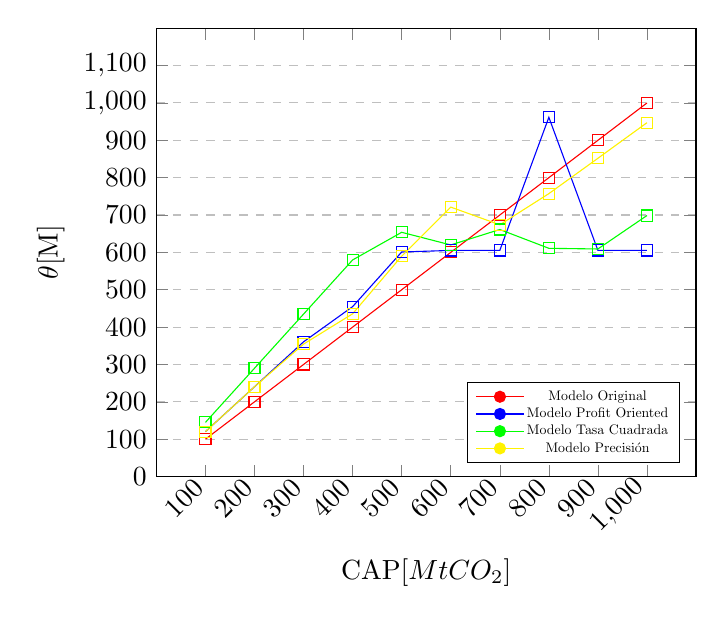
\begin{tikzpicture}
\centering
\begin{axis}[legend style={nodes={scale=0.5, transform shape}}, 
        legend image post style={mark=*},
    xlabel={CAP[$MtCO_2$]},
    ylabel={$\theta$[M]},
    xmin=0, xmax=1100,
    ymin=0, ymax=1200,
    xtick={100,200,300,400,500,600,700,800,900,1000},
    xticklabel style = {rotate=45,anchor=east},
    ytick={0,100,200,300,400,500,600,700,800,900,1000,1100},
    legend pos=south east,
    ymajorgrids=true,
    grid style=dashed,
]

\addplot[
    color=red,
    mark=square,
    ]
    coordinates {
    (100,100)(200,200)(300,300)(400,400)(500,500)(600,600)(700,700)(800,800)(900,900)(1000,1000)
    };

\addplot[
    color=blue,
    mark=square,
    ]
    coordinates {(100,120.2)(200,240.4)(300,360.6)(400,454.79)(500,601)(600,605.27)(700,605.27)(800,961.6)(900,605.27)(1000,605.27)
    };
    
\addplot[
    color=green,
    mark=square,
    ]
    coordinates {
    (100,144.94)(200,289.88)(300,434.83)(400,579.77)(500,653.75)(600,619.93)(700,661.25)(800,610.91)(900,609.12)(1000,698.67)
    };
    
\addplot[
    color=yellow,
    mark=square,
    ]
    coordinates {
    (100,120.2)(200,240.4)(300,354.5)(400,435.64)(500,590.04)(600,721.2)(700,673.83)(800,757.24)(900,851.9)(1000,947.17)
    }; 
    \legend{Modelo Original, Modelo Profit Oriented,Modelo Tasa Cuadrada,Modelo Precisión}

\end{axis}
\end{tikzpicture}
}
\caption{{\footnotesize Permisos emitidos por CAP}}
\label{permisospormodelo}
\end{figure}

\begin{figure}[H]
\centering
\resizebox{12cm}{9cm}{%
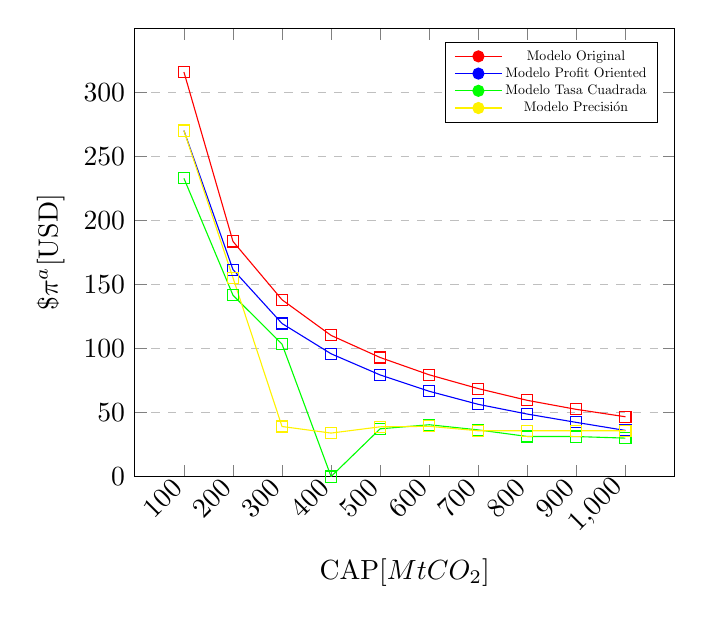
\begin{tikzpicture}
\centering
\begin{axis}[legend style={nodes={scale=0.5, transform shape}}, 
        legend image post style={mark=*},
    xlabel={CAP[$MtCO_2$]},
    ylabel={$\$ \pi^a$[USD]},
    xmin=0, xmax=1100,
    ymin=0, ymax=350,
    xtick={100,200,300,400,500,600,700,800,900,1000},
    xticklabel style = {rotate=45,anchor=east},
     ytick={0,50,100,150,200,250,300},
    legend pos=north east,
    ymajorgrids=true,
    grid style=dashed,
]

\addplot[
    color=red,
    mark=square,
    ]
    coordinates {
    (100,315.82)(200,183.55)(300,138.01)(400,110.18)(500,92.93)(600,79.42)(700,68.65)(800,59.48)(900,52.43)(1000,46.66)
    };

\addplot[
    color=blue,
    mark=square,
    ]
    coordinates {(100,270.12)(200,161.56)(300,119.47)(400,95.83)(500,79.31)(600,66.57)(700,56.37)(800,48.76)(900,42.26)(1000,35.98)

    };
    
\addplot[
    color=green,
    mark=square,
    ]
    coordinates {
    (100,232.82)(200,141.55)(300,103.32)(400,0)(500,37.26)(600,40.43)(700,36.41)(800,31.27)(900,31.21)(1000,30)

    };
    
\addplot[
    color=yellow,
    mark=square,
    ]
    coordinates {
    (100,270.12)(200,155.15)(300,39.06)(400,33.93)(500,38.82)(600,39.2)(700,35.73)(800,35.73)(900,35.73)(1000,35.73)


    }; 
    \legend{Modelo Original, Modelo Profit Oriented,Modelo Tasa Cuadrada,Modelo Precisión}

\end{axis}
\end{tikzpicture}
}
\caption{{\footnotesize Precio de venta de permisos $\pi^a$ por CAP}}
\label{permisospormodelo}
\end{figure}

\begin{figure}[H]
\centering
\resizebox{12cm}{9cm}{%
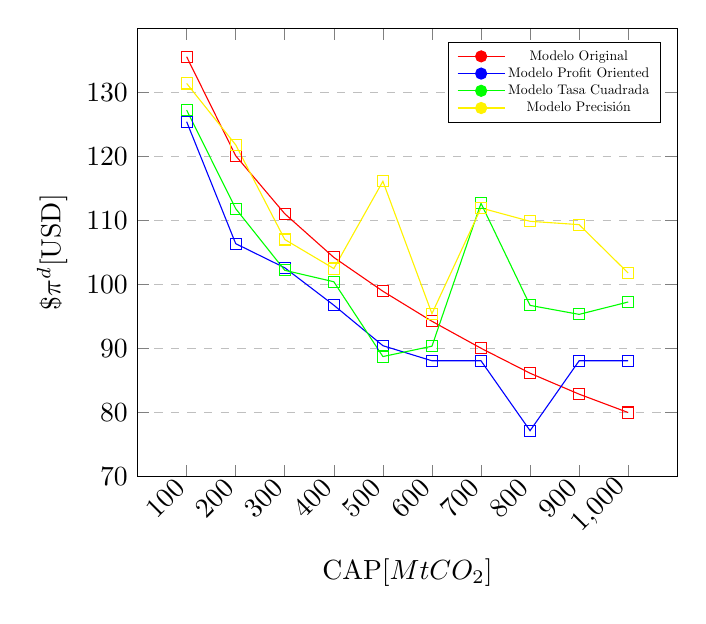
\begin{tikzpicture}
\centering
\begin{axis}[legend style={nodes={scale=0.5, transform shape}}, 
        legend image post style={mark=*},
    xlabel={CAP[$MtCO_2$]},
    ylabel={$\$ \pi^d$[USD]},
    xmin=0, xmax=1100,
    ymin=70, ymax=140,
    xtick={100,200,300,400,500,600,700,800,900,1000},
    xticklabel style = {rotate=45,anchor=east},
     ytick={70,80,90,100,110,120,130},
    legend pos=north east,
    ymajorgrids=true,
    grid style=dashed,
]

\addplot[
    color=red,
    mark=square,
    ]
    coordinates {
    (100,135.54)(200,120.08)(300,111.03)(400,104.21)(500,98.93)(600,94.24)(700,90.03)(800,86.13)(900,82.86)(1000,79.99)

    };

\addplot[
    color=blue,
    mark=square,
    ]
    coordinates {
    (100,125.4)(200,106.36)(300,102.59)(400,96.75)(500,90.43)(600,88.07)(700,88.07)(800,77.16)(900,88.07)(1000,88.07)

    };
    
\addplot[
    color=green,
    mark=square,
    ]
    coordinates {
    (100,127.22)(200,111.82)(300,102.2)(400,100.41)(500,88.73)(600,90.35)(700,112.66)(800,96.72)(900,95.32)(1000,97.25)
    };
    
\addplot[
    color=yellow,
    mark=square,
    ]
    coordinates {
    (100,131.38)(200,121.78)(300,107.01)(400,102.47)(500,116.1)(600,95.43)(700,111.93)(800,109.85)(900,109.33)(1000,101.77)
    }; 
    \legend{Modelo Original, Modelo Profit Oriented,Modelo Tasa Cuadrada,Modelo Precisión}

\end{axis}
\end{tikzpicture}
}
\caption{{\footnotesize Promedio precios de electricidad (2019-2050) $\pi^d$ por CAP}}
\label{permisospormodelo}
\end{figure}


REVISAR SI LOS PID POR MODELO Y VER CUAL ES EL MEJOR, CREO QUE LOS MODELOS NUEVOS SON MEJORES CON POCO CAP PERO CON MAS CAP EL ORIGINAL ES MEJOR